% ************************** Thesis Chapter3 **********************************
\chapter{ระเบียบวิธีวิจัย}
ในการทําโครงการวิจัยแอพพลิเคชั่นสำหรับวิเคราะห์วิดีโอ(video analytics) จะมีการทำงานหลากหลายส่วนมาทำงานร่วมกัน ซึ่งทำให้จำเป็นจะต้องมีระเบียบวิจัยสำหรับอธิบายภาพรวม
\subsection*{โดยในระเบียบวิจัยนี้จะมีหัวข้อ และระเบียบวิธีวิจัยดังนี้}
\begin{itemize}\setlength\itemsep{-0.3em}
	\item แผนการดำเนินงาน
	\item เครื่องมือที่ใช้ในการดำเนินงานวิจัย
	\item ภาพรวมของแอพพลิเคชั่น
	\item รายละเอียดของโมเดล
\end{itemize}
\vspace{3mm}
\section{หน้าที่ความรับผิดชอบ} 
\paragraph*{ปฐมพงศ์ สินธุ์งาม}
สร้างและทดสอบโมเดล I3D และ ทำโปรแกรมในส่วน tracking
\paragraph*{ศุภกร เบญจวิกรัย}
รวบรวมฟังก์ชั่นต่างๆของแอพพลิเคชั่น และ ทำแอพพลิเคชั่นในส่วน selection , detection
\paragraph*{อุกฤษฎ์ เลิศวรรณาการ}
สร้างและทดสอบโมเดล Resnet-50 และ ทำโปรแกรมในส่วน person reid 

\vspace{3mm}
\section{แผนการดำเนินงาน}
โดยจากที่กล่าวไปตอนต้นในบทนำ
การดำเนินงานและการออกแบบการสร้างหุ่นยนต์ฮิวมานอยด์ UTHAI มีแผนการทำงานซึ่งแบ่งออกเป็นสามส่วนดังนี้
ส่วนแรกคือ ส่วนของฮาร์ดแวร์ที่เกี่ยวกับโครงสร้างทางกลของหุ่นยนต์ฮิวมานอยด์ เช่น ข้อต่อ ก้านต่อ ฝ่าเท้า
รวมไปถึงระบบอิเล็กทรอนิกส์ ตัวประมวลผลการควบคุม เซนเซอร์ ตัวขับเคลื่อนต่าง ๆ และส่วนที่สองคือ
ส่วนของซอฟท์แวร์ที่เกี่ยวข้องกับการติดต่อสื่อสารกันเบื้องต้น การควบคุมตัวขับเคลื่อนที่ข้อต่อ การอ่านค่าเซนเซอร์
และส่วนที่สาม คือระบบพื้นฐานสำหรับการนำไปศึกษาและพัฒนา โดยจะครอบคลุมไปถึงเอกสารวิธีการใช้งานในรูปแบบออนไลน์

ในการเริ่มทำงานวิจัยที่เกี่ยวกับฮิวมานอยด์นั้นสิ่งจำเป็นที่ต้องทำในอันดับแรกคือการศึกษาสิ่งที่เคยมีอยู่ หรืองานวิจัยมีนักวิจัยอื่นที่ทำเอาไว้แล้ว
จากนั้นศึกษาทำความเข้าใจใน ข้อดี-ข้อเสีย ของวิธีหรือกระบวนการต่างๆ เพื่อนำมาประยุกต์ใช้กับหุ่นยนต์ฮิวมานอยด์ภายในงานวิจัยนี้
ในการศึกษาโครงสร้างทางกลและระบบของหุ่นยนต์ฮิวมานอยด์ที่มีอยู่แล้วสิ่งที่ต้องดูและให้ความสนใจเป็นพิเศษคือ
วิธีการเชื่อมต่อกันระหว่างก้านต่อและข้อต่อ, ลักษณะโครงสร้างที่สามารถทำให้เกิดการเคลื่อนไหวเพียงพอต่อการเดิน,
ตำแหน่งที่ใช้ในติดตั้งเซนเซอร์หรือตัวรับรู้ต่างๆ, การเลือกใช้วัสดุให้เหมาะสม
และการทำงานของเซนเซอร์และตัวขับเคลื่อนที่จำเป็นต้องใช้ในการควบคุมการทำงานของหุ่นยนต์
เมื่อเราทำความศึกษาเสร็จเรียบร้อยแล้ว จึงเริ่มดำเนินงานวิจัยการพัฒนาโครงสร้างและระบบพื้นฐาน
ในส่วนนี้ทางกลจะเป็นการออกแบบโครงสร้างและจัดสร้างขึ้นมา ทางซอฟต์แวร์จะเป็นการสร้างแบบจำลองของหุ่นยนต์
ระบบจำลองที่สามารถจำลองการทำงานของหุ่นยนต์ได้ และติดต่อส่วนของทางกลกับทางโปรแกรม
สุดท้ายระบบพื้นฐานจะออกแบบโครงสร้างระบบพื้นฐานเพื่อทำให้เกิดการพัฒนาต่อได้อย่างมีประสิทธิภาพ
ในบทนี้ก็จะกล่าวถึงกระบวนการออกแบบและการดำเนินการตามแผนที่วางเอาไว้

\clearpage
\section{การออกแบบโครงสร้างของหุ่นยนต์}
การออกแบบทางโครงสร้างทางกลของหุ่นยนต์ฮิวมานอยด์ UTHAI นั้น ผู้วิจัยได้เลือกใช้โปรแกรมออกแบบโครงสร้างเป็นโปรแกรม Solidworks
ที่ช่วยในการพัฒนาแบบจำลองของหุ่นยนต์ฮิวมานอยด์ UTHAI
เนื่องจากโปรแกรม Solidworks เป็นโปรแกรมที่ใช้ในการออกแบบ และวาดแบบทางวิศวกรรม
สามารถวิเคราะห์โครงสร้างการรับแรงของแบบจำลองได้ อีกทั้งยังเป็นเครื่องมือที่มีการใช้งานอย่างแพร่หลาย
ทำให้สามารถดาวน์โหลดแบบจำลองต่างๆที่มีคนพัฒนาเข้าเข้ามาใช้ร่วมกับการออกแบบได้ 
และด้วยทางผู้วิจัยมีความคำนึงถึงการพัฒนา ต่อยอดเป็นหลัก ดังนั้นการออกโครงสร้างทางกลของหุ่นยนต์ฮิวมานอยด์ UTHAI
จึงถูกออกแบบมาเพื่อให้สามารถรองรับการปรับเปลี่ยน เปลี่ยนแปลง แก้ไขชิ้นส่วนต่างๆของตัวหุ่นยนต์ฮิวมานอยด์ UTHAI ต่อไปได้

\subsection{โครงสร้างของหุ่นยนต์ฮิวมานอยด์ UTHAI}
หุ่นยนต์ฮิวมานอยด์ที่สร้างขึ้นประกอบด้วยส่วนของลำตัวและส่วนขา ในขาแต่ละข้างออกแบบให้ข้อต่อมีเป็นลักษณะของข้อต่อแบบหมุน (Revolute joint)
เพื่อเลียนแบบโครงสร้างของมนุษย์ที่ประกอบด้วย ส่วนของสะโพกที่มีองศาอิสระจำนวน 3 องศาอิสระ หัวเข่า 1
องศาอิสระ และข้อเท้า 2 องศาอิสระ รวมทั้งขาข้างละ 6 องศาอิสระ ระบบต้นกำลังที่ใช้ในแต่ละข้อต่อเป็นดิจิตอลเซอร์โว
การออกแบบหุ่นยนต์ฮิวมานอยด์ UTHAI นั้น
สิ่งแรกที่ต้องทำ คือ การกำหนดโครงสร้างของข้อต่อและก้านต่อ ดังรูปที่ \ref{fig:uthai_design_structure}
ซึ่งโครงสร้างนั้นทางผู้วิจัยได้อ้างอิงมาจากสัดส่วนของมนุษย์จริง
และมีจุดศูนย์กลางมวลอยู่บริเวณกระดูกเชิงกรานของตัวหุ่นยนต์ฮิวมานอยด์เอง ดังรูปที่ \ref{fig:uthai_structure1}

\begin{figure}[!ht]
    \centering
    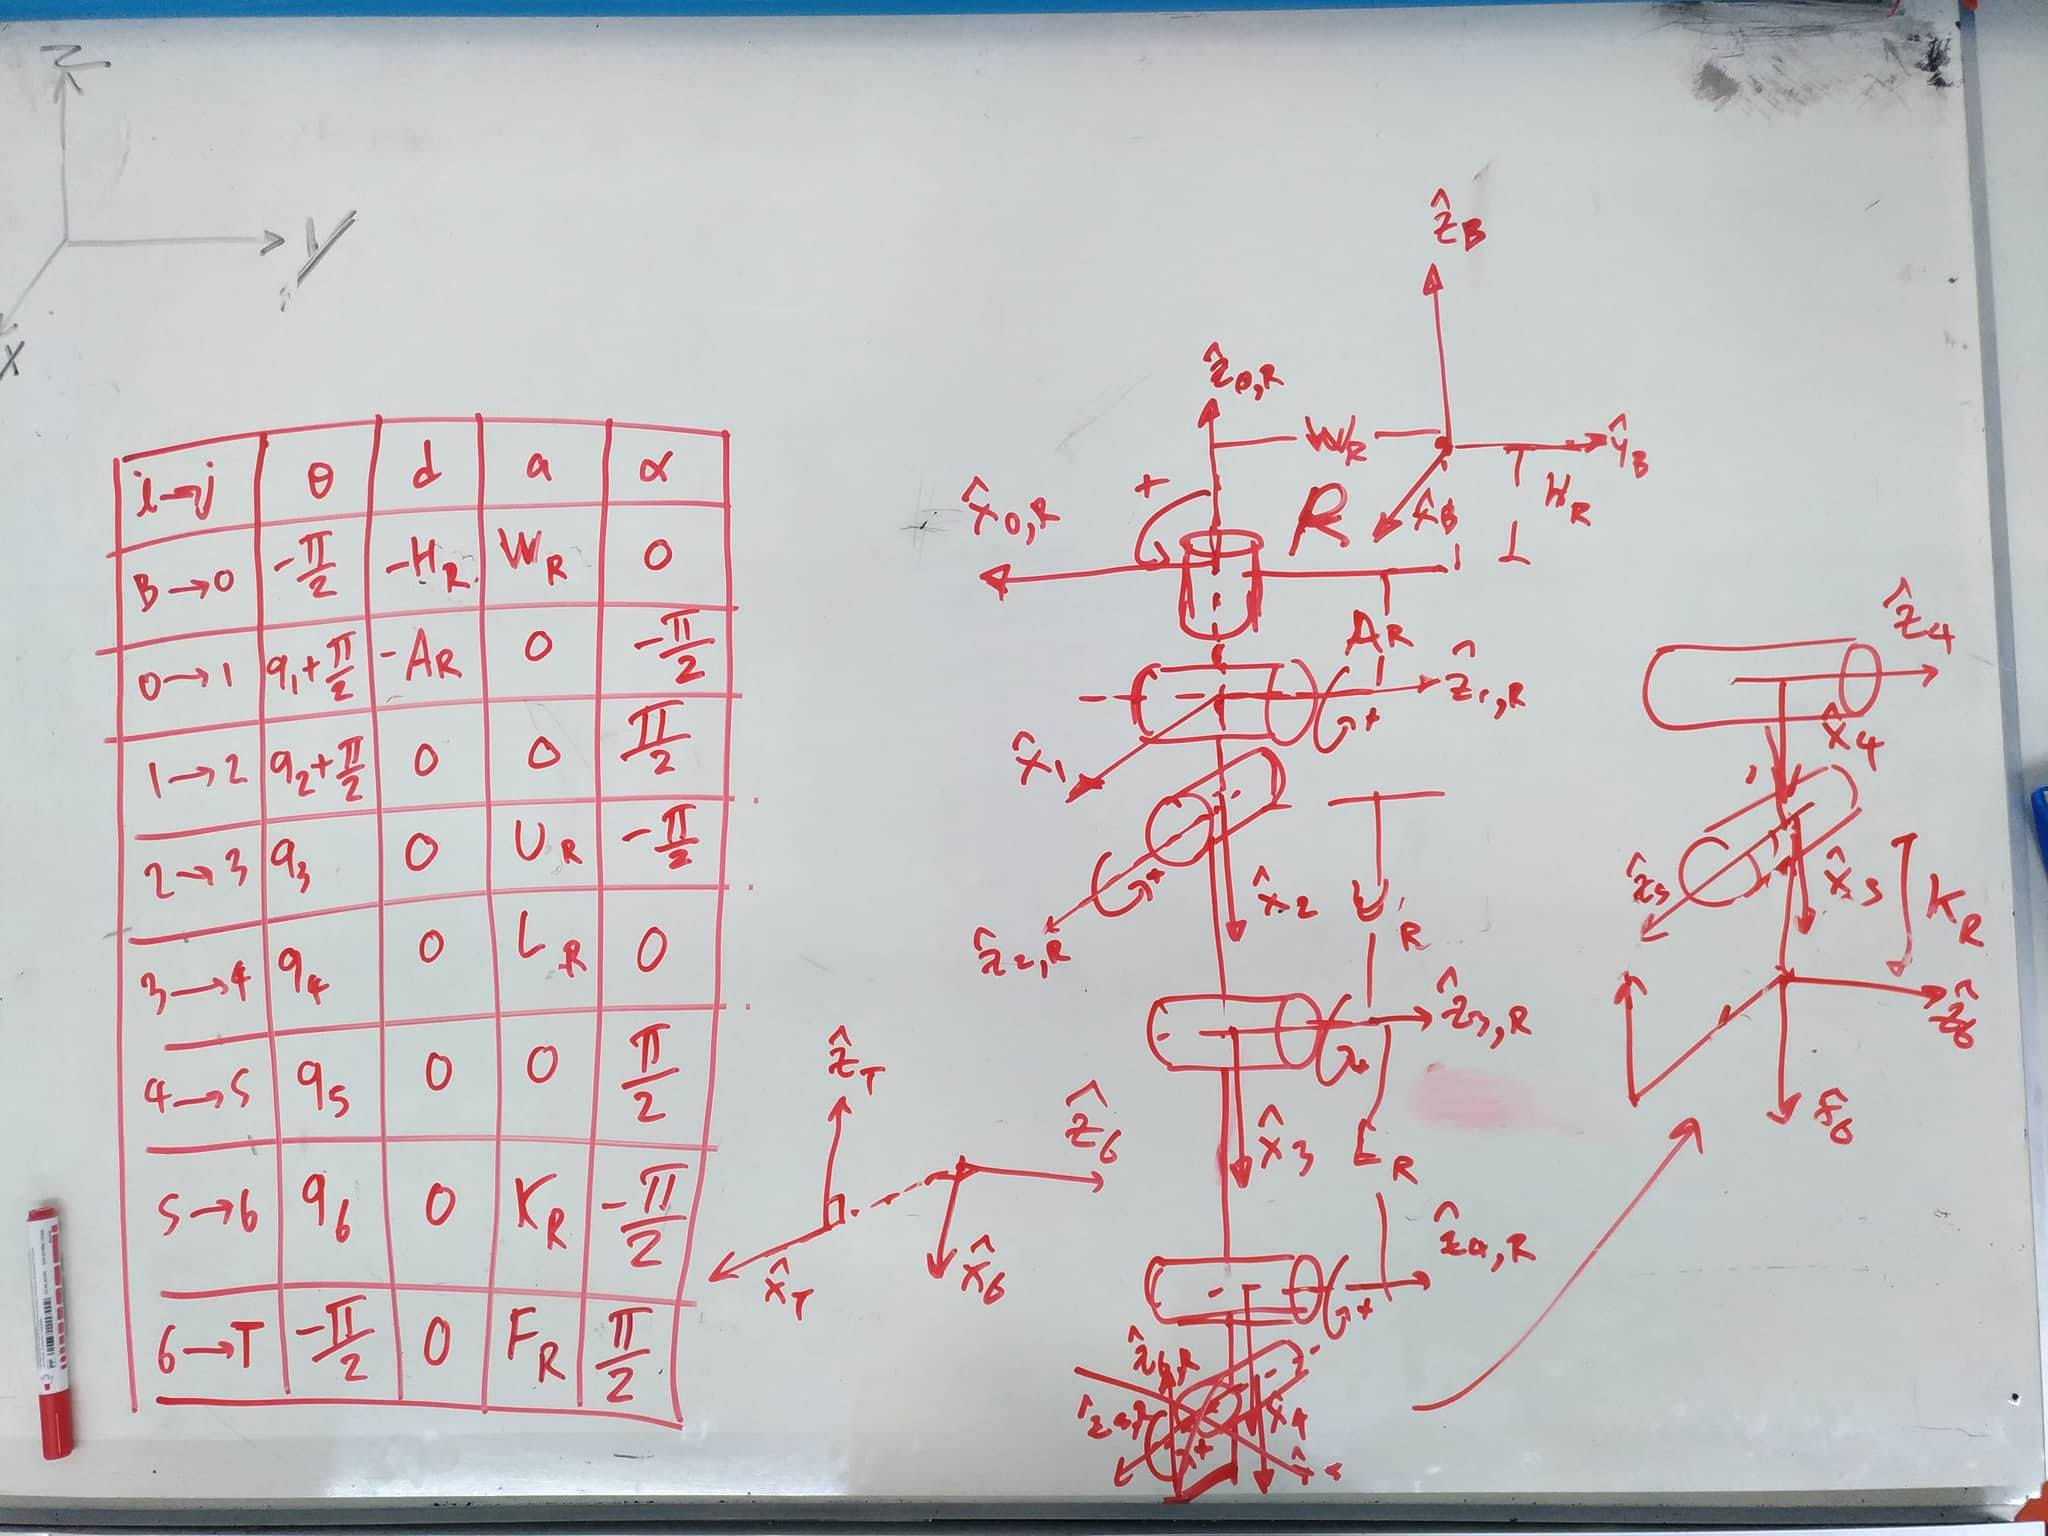
\includegraphics[width=0.5\textwidth]{chapter3/images/clean/uthai_design_structure.jpg}
    \caption{การออกแบบโครงสร้างของหุ่นยนต์ UTHAI}
    \label{fig:uthai_design_structure}
\end{figure}

\begin{figure}[!ht]
    \centering
    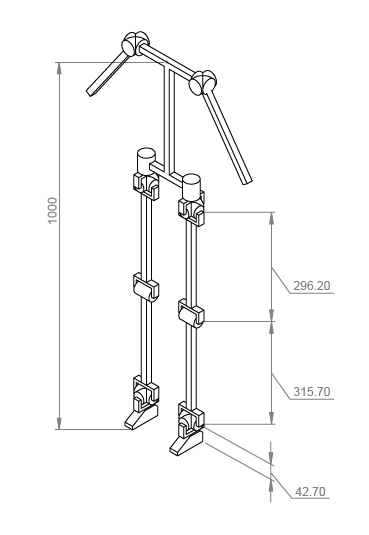
\includegraphics[width=0.35\textwidth]{chapter3/images/uthai_structure1.png}
    \caption{ภาพแสดงแสดงโครงสร้างของหุ่นยนต์ UTHAI}
    \label{fig:uthai_structure1}
\end{figure}

เมื่อเราได้แบบของหุ่นยนต์ฮิวมานอยด์ UTHAI แล้ว ลำดับต่อไปคือการกำหนดตำแหน่งการติดตั้งเซนเซอร์และตัวขับเคลื่อนต่างๆเข้าไป
โดยมีเซนเซอร์ตรวจการสัมผัสพื้นติดตั้งที่ใต้ฝ่าเท้าของหุ่นยนต์ เซนเซอร์หน่วยวัดความเฉื่อยติดตั้งไว้บริเวณลำตัวของหุ่นยนต์ฮิวมานอยด์
และที่ข้อต่อในแต่ละจุดใช้ตัวขับเคลื่อนเป็นดิจิตอลเซอร์โว ดังรูปที่ \ref{fig:uthai_structure2}

\begin{figure}[!ht]
    \centering
    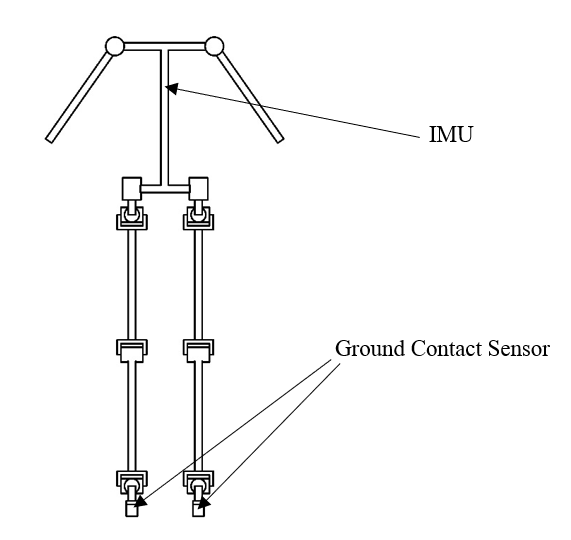
\includegraphics[width=0.5\textwidth]{chapter3/images/uthai_sensor.PNG}
    \caption{ภาพแสดงการติดตั้งเซนเซอร์ในจุดต่างๆ}
    \label{fig:uthai_structure2}
\end{figure}

ส่วนวัสดุที่ใช้ทำโครงสร้างหุ่นยนต์ฮิวมานอยด์ UTHAI ทางผู้วิจัยเลือกใช้วัสดุหลักเป็น PLA ที่ขึ้นรูปด้วยวิธีการขึ้นรูปสามมิติ
ก้านต่อเป็นคาร์บอนไฟเบอร์ เนื่องจากจะทำให้โครงสร้างมีน้ำหนักเบา ขึ้นรูปได้สะดวกทำให้สามารถปรับปรุงแก้ไขง่าย
และมีวัสดุเสริมบางชิ้นส่วนที่ทำจากอลูมิเนียมเนื่องจากต้องการความแข็งแรงมาก ดังตารางที่ \ref{tab:material_properties}

\begin{table}[!ht]
	\centering
	\begin{tabular}{| l | l | l |}
		\hline
		Material & Longitudinal Tensile Strength ($ksi$) & Density ($g/cm^3$) \\
        \hline
        Carbon Fiber & 300 & 1.55 \\
        Steel & 100	& 7.7 \\
        Titanium & 120 & 4.34 \\
        Aluminum & 35 & 2.7 \\
        PLA 3D printing (50 \% infill) & 3.5 & 1.26 \\
        PLA 3D printing (100 \% infill) & 5.5 & 1.26 \\
	    \hline
	\end{tabular}
	\caption{ตารางแสดงสมบัติทางกลของวัสดุต่าง ๆ}
	\label{tab:material_properties}
\end{table}

\clearpage
\subsection{การจัดทำชิ้นส่วนโครงสร้างของหุ่นยนต์ฮิวมานอยด์ UTHAI}
ในกาารจัดทำชิ้นส่วนโครงสร้างของหุ่นยนต์ฮิวมานอยด์อุทัยนั้นทาง ผู้วิจัยได้คำนึงถึงความแข็งแรงเป็นหลักซึ่งมีความสำคัญมาก
ในการเคลื่อนที่ของหุ่นยนต์ อีกทั้งยังต้องมีน้ำหนักที่เบาเพื่อประหยัดพลังงานที่ต้องใช้ในการขับเคลื่อน\footnote{ Printing Guide [https://filaments.ca/pages/temperature-guide]}
ดังนั้นผู้วิจัยจึงได้ใช้การขึ้นรูปชิ้นงานด้วยเทคนิคการพิมพ์สามมิติ โดยจะใช้วัสดุหลักเป็นพลาสติก PLA ซึ่งมีความแข็งมากกว่าและขึ้นรูปง่ายกว่าพลาสติกชนิด ABS ดังตารางที่ \ref{tab:plastic_material_properties}
และก้านต่อเป็นคาร์บอนไฟเบอร์ เพื่อให้ตอบโจทย์กับหุ่นยนต์แพลตฟอร์มเพื่อพัฒนาต่อยอดในอนาคต
ซึ่งผู้ใช้ทุกคนสามารถพิมพ์ชิ้นงานขึ้นมาได้ด้วยตนเอง\footnote{ PLA vs ABS [https://www.3dhubs.com/knowledge-base/pla-vs-abs-whats-difference]}

\begin{table}[!ht]
	\centering
	\begin{tabular}{| l | l | l |}
		\hline
		Properties & ABS & PLA \\
        \hline
        Tensile Strength & 27 $MPa$ & 37 $MPa$ \\
        Elongation & 3.5 \- 50\% & 6\% \\
        Flexural Modulus & 2.1 \- 7.6 $GPa$ & 4 $GPa$ \\
        Density & 1.0 - 1.4 $g/cm^3$ & 1.3 $g/cm^3$ \\
        Melting Point & 230$°C$ - 240$°C$ & 215$°C$ - 235$°C$ \\ 
        การย่อยสลายทางธรรมชาติ & ไม่ได้ & ได้ (ภายใต้เงื่อนไขที่ถูกต้อง) \\
	    \hline
	\end{tabular}
	\caption{ตารางแสดงสมบัติทางกลของวัสดุพลาสติก}
	\label{tab:plastic_material_properties}
\end{table}

แต่เนื่องจากในปัจจุบันนี้เครื่องพิมพ์สามมิติส่วนมากจะไม่รองรับการพิมพ์ชิ้นงานที่มีขนาดใหญ่ ซึ่งมีขนาดมากกว่า
30x30x30 ซม. (กว้างxยาวxสูง) ดังนั้นชิ้นงานที่ขึ้นรูป ที่มีขนาดใหญ่เกินกว่านี้อาจจะต้องทำการตัดชิ้นงานออกเป็นส่วนย่อยๆก่อน
แล้วจึงค่อยนำมาประกอบรวมกันทีหลังอีกครั้งหนึ่ง โดยพื้นที่ทำการพิมพ์ของเครื่องพิมพ์สามมิติที่มีวางจำหน่าย\footnote{The truth about 3D printer maximum print areas [https://www.zdnet.com/article/what-manufacturers-dont-want-you-to-know-the-truth-about-3d-printer-maximum-print-areas/]}
และใช้งานแพร่หลายในท้องตลาดแสดง ดังตารางที่ \ref{tab:3dprint_space} 
\begin{table}[!ht]
	\centering
	\begin{tabular}{| l | l | l | l |}
		\hline
		ชื่อเครื่องพิมพ์สามมิติ & ขนาดความกว้าง (มม.) & ขนาดความลึก (มม.) & ขนาดความสูง (มม.) \\
        \hline
        MakerBot Replicator+ & 292 & 192 & 165 \\
        Ultimaker 3 & 188 & 185 & 200 \\
        LulzBot Mini & 152 & 152 & 158 \\
        Dreammaker Overlord Pro Plus & 79 & 79 & 255 \\
        New Matter MOD-t & 145 & 95 & 125 \\
	    \hline
	\end{tabular}
	\caption{ตารางแสดงขนาดของชิ้นงานที่สามารถพิมพ์ได้ในเครื่องพิมพ์ชนิดต่างๆ}
	\label{tab:3dprint_space}
\end{table}



%%%%%%%%%%%%%%%%%%%%%%%%%%%%%%%%%%%%%%%%%%%%%%%%%%%%%%%%%%%%%%%%%%%%%%%%%%%%%%%
%%%%%%%%%%%%%%%%%%%%%%%%%%%%%%%%%%%%%%%%%%%%%%%%%%%%%%%%%%%%%%%%%%%%%%%%%%%%%%%
%%%%%%%%%%%%%%%%%%%%%%%%%%%%%%%%%%%%%%%%%%%%%%%%%%%%%%%%%%%%%%%%%%%%%%%%%%%%%%%
\clearpage
\subsection{อุปกรณ์ที่ใช้ในหุ่นยนต์ฮิวมานอยด์ UTHAI}

\subsubsection*{Dynamixel Servo EX-106+}
Dynamixel EX-106+ เป็นตัวขับเคลื่อนที่นิยมใช้ในหุ่นยนต์ปัจจุบัน ซึ่งเป็นเซอร์โวมอเตอร์ที่เหมาะสำหรับทำหุ่นยนต์โดยเฉพาะ
ภายในประกอบไปด้วย มอเตอร์กระแสตรง ชุดเฟืองมอเตอร์ ไดรเวอร์คอนโทรเลอร์ สามารถเชื่อมต่อกันผ่านบัส RS-485
\footnote{ Robot Actuator [http://support.robotis.com/en/product/actuator/dynamixel/ex\_series/ex-106.htm] }
มีการควบคุมตำแหน่งและความเร็วด้วย PID ภายในมีเซนเซอร์สามารถที่จะอ่านค่าความเร็ว
แรงดันไฟฟ้า กระแสไฟฟ้า อุณหภูมิ ตำแหน่ง และแรงบิดจากมอเตอร์ทุกตัวได้ แต่ละมอเตอร์แต่ละตัวจะมีบอร์ดควบคุมของตัวเอง
เราสามารถที่จะจ่ายไฟให้มอเตอร์และควบคุมผ่าน Serial ได้ ดังรูปที่ \ref{fig:dxl_ex106}
การทำงานของตัวดิจิตอลเซอร์โวนี้สามารถทำได้ 2 รูปแบบ\footnote{ EX-106+ Mode [http://www.trossenrobotics.com/dynamixel-ex-106-robot-actuator.aspx]}
คือ

\paragraph*{Joint Mode}
สามารถที่จะควบคุมแรงบิด ความเร็ว และตำแหน่งได้ ความละเอียดในการควบคุมตำแหน่งอยู่ที่ 10bit (0-1023) หมุนได้อยู่ในช่วง -150 ถึง 150 องศา

\paragraph*{Wheel Mode}
สามารถที่จะควบคุมแรงบิด ความเร็ว และทิศทางได้ ความละเอียดของความเร็วอยู่ที่ 10bit (0-1023) สามารถหมุนได้ครบ 360 องศาได้ ความเร็วสูงสุดอยู่ที่ 114 RPM

\begin{figure}[!ht]
    \centering
    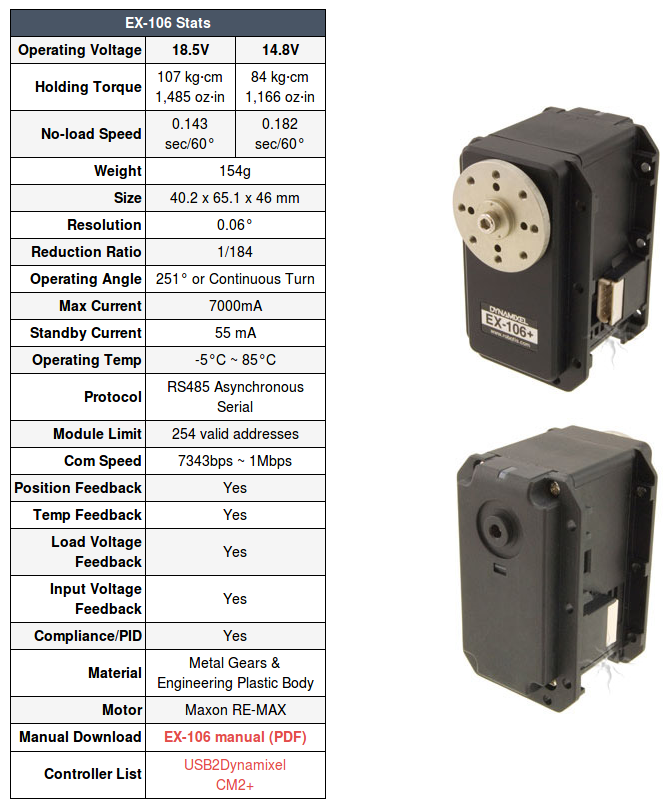
\includegraphics[width=0.7\textwidth]{chapter3/images/dxl_ex106.png}
    \caption{แสดงประสิทธิภาพของมอเตอร์ EX-106+}
    \label{fig:dxl_ex106}
\end{figure}


\clearpage
\subsubsection*{USB2Dynamixel}
USB2Dynamixel เป็นอุปกรณ์สำหรับเชื่อมต่อดิจิตอลเซอร์โว กับหน่วยประมวลผลระดับสูง (Odroid) โดยจะเชื่อมต่อผ่านพอร์ท USB
ที่อยู่บน Odroid และแปลงให้ส่งข้อมูลไปยังดิจิตอลเซอร์โวผ่านสาย 2 เส้น คือ D+ และ D- ดังรูปที่ \ref{fig:dynamixel2pc}
เป็นการเชื่อมต่อแบบ RS-485\footnote{USB2Dynamixel [http://support.robotis.com/en/product/auxdevice/interface/usb2dxl\_manual.html]}
ืทำให้สามารถส่งข้อมูลไปยังหลายๆอุปกรณ์บนสายเส้นเดียวได้
และสามารถส่งในระยะทางไกลๆได้\footnote{http://support.robotis.com/en/images/product/auxdevice/interface/}


\begin{figure}[!ht]
    \centering
    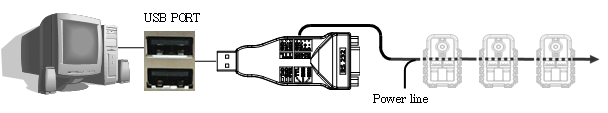
\includegraphics[width=0.75\textwidth]{chapter3/images/dynamixel2pc.png}
    \caption{ภาพแสดงการติดต่อสื่อสารระหว่างคอมพิวเตอร์กับดิจิตอลเซอร์โว}
    \label{fig:dynamixel2pc}
\end{figure}

ในการใช้งาน ผู้ใช้งานจำเป็นต้องเลือกรูปแบบการติดต่อสื่อสารซึ่งแต่ละรูปแบบก็จะมีลักษณะการเชื่อมต่อที่แตกต่างกันไป
USB2Dynamixel ได้แบ่งการติดต่อสื่อสารออกเป็น 3 รูปแบบ\footnote{http://support.robotis.com/en/product/auxdevice/interface/usb2dxl\_manual.htm}คือ
ดังรูปที่ \ref{fig:useusb2dynamixel}
\vspace{-10pt}
\begin{enumerate}[label=\arabic*, leftmargin=1.5cm]
    \setlength\itemsep{-0.25em}
    \item TTL Communication : สำหรับดิจิตอลเซอร์โวที่ใช้พอร์ทชนิด 3-pin ในตระกูล AX Series
    \item RS485 Communication : สำหรับดิจิตอลเซอร์โวที่ใช้พอร์ทชนิด 4-pin ในตระกูล DX Series
    \item RS232 Communication : ใช้สำหรับติดต่อสื่อสารกับคอนโทรลเลอร์ผ่านสายเคเบิล
\end{enumerate}
\vspace{-15pt}
\begin{figure}[!ht]
    \centering
    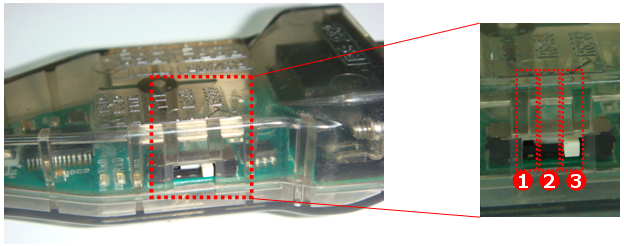
\includegraphics[width=0.5\textwidth]{chapter3/images/useusb2dynamixel.png}
    \caption{ภาพแสดงการเลือกโหมดใช้งานของ USB2Dynamixel}
    \label{fig:useusb2dynamixel}
\end{figure}

แต่จากการทดลองนำมาใช้ ผู้วิจัยพบว่าดิจิตอลที่ใช้ในการทำงานวิจัยครั้งนี้เป็นชนิด 4-pin ซึ่งใช้ RS485 ในการติดต่อสื่อสาร
ด้วยขนาดของตัว USB2Dynamixel มีขนาดที่ใหญ่ทำให้การทำงานมีความลำบากในการติดตั้งลงบนตัวของหุ่นยนต์ฮิวมานอยด์อุทัย
จึงได้ทำการเปลี่ยนเป็น USB2RS485\footnote{https://softgenie.dk/diverse/280-usb2rs485.html}
\begin{figure}[!ht]
    \centering
    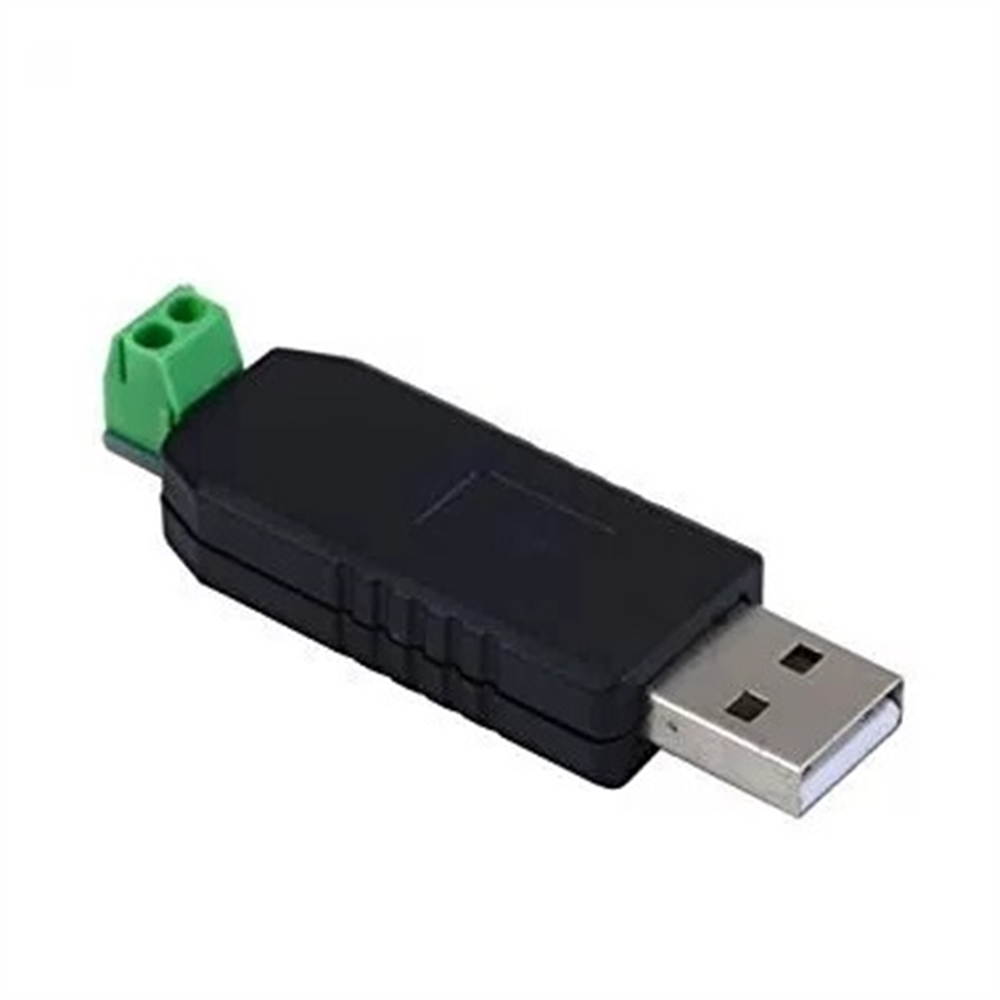
\includegraphics[width=0.25\textwidth]{chapter3/images/usb2rs485.jpg}
    \caption{USB2RS485 Module}
    \label{fig:usb2rs485}
\end{figure}

\clearpage
\subsubsection*{Inertial Measurement Unit (IMU)}
ผู้วิจัยได้เลือกใช้เซนเซอร์หน่วยวัดความเฉื่อยเป็น MPU-9250 ดังรูปที่ \ref{fig:mpu9250} มาใช้ในการอ่านหาค่ามุมเอียงของฐานหุ่นยนต์ฮิวมานอยด์อุทัย
เพื่อใช้ในการคุมเสถียรภาพของหุ่นยนต์
โดยเซนเซอร์ตัวนี้สามารถวัดค่าได้ 9 แกนคือ วัดค่าความเร็วเชิงมุม (gyroscope) 3 แกน วัดค่าความเร่งเชิงเส้น (accelerometer) 3 แกน
และวัดค่าสนามแม่เหล็กโลก (magnetometer) 3 แกน ซึ่งเซนเซอร์จะติดตั้งบริเวณส่วนของลำตัวหุ่นยนต์ฮิวมานอยด์อุทัย
เนื่องจากว่าจะเป็นจุดที่สามารถบ่งบอกได้ถึงการเคลื่อนที่และมุมเอียงของหุ่นยนต์ในขณะนั้นได้\footnote{ MPU-9250 [http://www.arduiner.com/en/gy-series-axis-accellerometers/6924-gy9255-mpu9255-sensor-module-alternative-mpu9150-mpu9250-3809200640200.html] }
\begin{figure}[!ht]
    \centering
    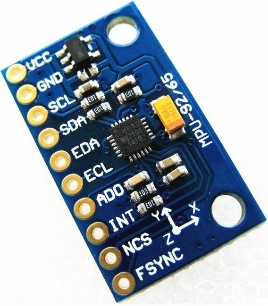
\includegraphics[width=0.2\textwidth]{chapter3/images/mpu9250.jpeg}
    \caption{แสดงเซนเซอร์ IMU MPU9250}
    \label{fig:mpu9250}
\end{figure}

\subsubsection*{Wi-Fi Adapter}
เนื่องจากหน่วยประมวลผลขั้นสูงของหุ่นยนต์ฮิวมานอยด์อุทัยนั้น ไม่สามารถเชื่อมต่อผ่านทาง Wifi ได้
จึงมีตัวรับสัญญาณ Wifi ดังรูปที่ \ref{fig:rpi_wifi_adaptor} ติดตั้งเพิ่มขึ้นมา เพื่อใช้ในการติดต่อสื่อสารระหว่างหน่วยประมวลผลระดับสูงที่ติดตั้งอยู่บนตัวของหุ่นยนต์
และคอมพิวเตอร์ที่เป็นตัวสั่งการซึ่งอยู่นอกตัวของหุ่นยนต์ ซึ่งในงานวิจัยนี้
จะใช้ส่งข้อมูลที่ได้หลังจากการประมวลผลบนคอมพิวเตอร์ไปยังตัวหุ่นยนต์ เช่น การวางแผนการเดิน การคำนวนพลศาสตร์ของหุ่นยนต์
และอื่นๆ โดยการส่งข้อมูลไปยังหน่วยประมวลผลระดับสูงจะมีตัวกลางในการรับส่งสัญญาณ
คือ ตัวกระจายสัญญาณ (Wifi router)\footnote{https://www.alzashop.com/tp-link-archer-c7-d470129.htm}
\begin{figure}[!ht]
    \centering
    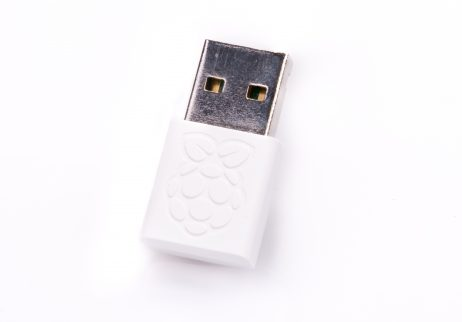
\includegraphics[width=0.3\textwidth]{chapter3/images/rpi_wifi_adaptor.jpg}
    \caption{ตัวรับสัญญาณ Wifi ของ RaspberryPi}
    \label{fig:rpi_wifi_adaptor}
\end{figure}
\begin{figure}[!ht]
    \centering
    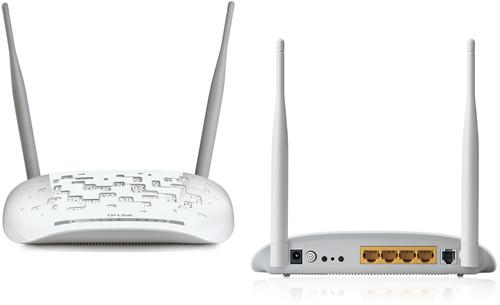
\includegraphics[width=0.3\textwidth]{chapter3/images/wifi_router.jpg}
    \caption{ตัวกระจายและรับส่งสัญญาณ wifi}
    \label{fig:wifi_router}
\end{figure}


\clearpage
\subsubsection*{Ground contact sensor}
เซนเซอร์ตรวจหน้าสัมผัสที่พื้นเป็นเซนเซอร์ที่ถูกติดตั้งบริเวณฝ่าเท้า เพื่อตรวจสอบการเดินของหุ่นยนต์ฮิวมานอยด์ว่าขณะนี้มีการสัมผัสของฝ่าเท้าของหุ่นยนต์กับพื้นหรือไม่ 
ซึ่งในงานวิจัยนี้ได้ใช้หลักการตัวตรวจจับแรงกดแบบค่าความต้านทานหรือ Force Sensing Resistor (FSR)
แนวคิดการออกแบบหลัก คือการออกแบบให้สามารถติดตั้งกับตัวหุ่นยนต์ได้เลย
ใช้ Arduino การพัฒนาซึ่งให้สามารถอ่านค่าได้ทั้งอนาลอคและดิจิตอลได้ อีกทั้งรองรับการต่อเซนเซอร์จำนวน 4 ตัว โดยมีลายวงจรดังรูปที่ \ref{fig:FSR_schematic}
และตัวอย่างของเซนเซอร์ตรวจจับหน้าสัมผัสดังรูป \ref{fig:complete_FSR}
\begin{figure}[!ht]
  \centering
  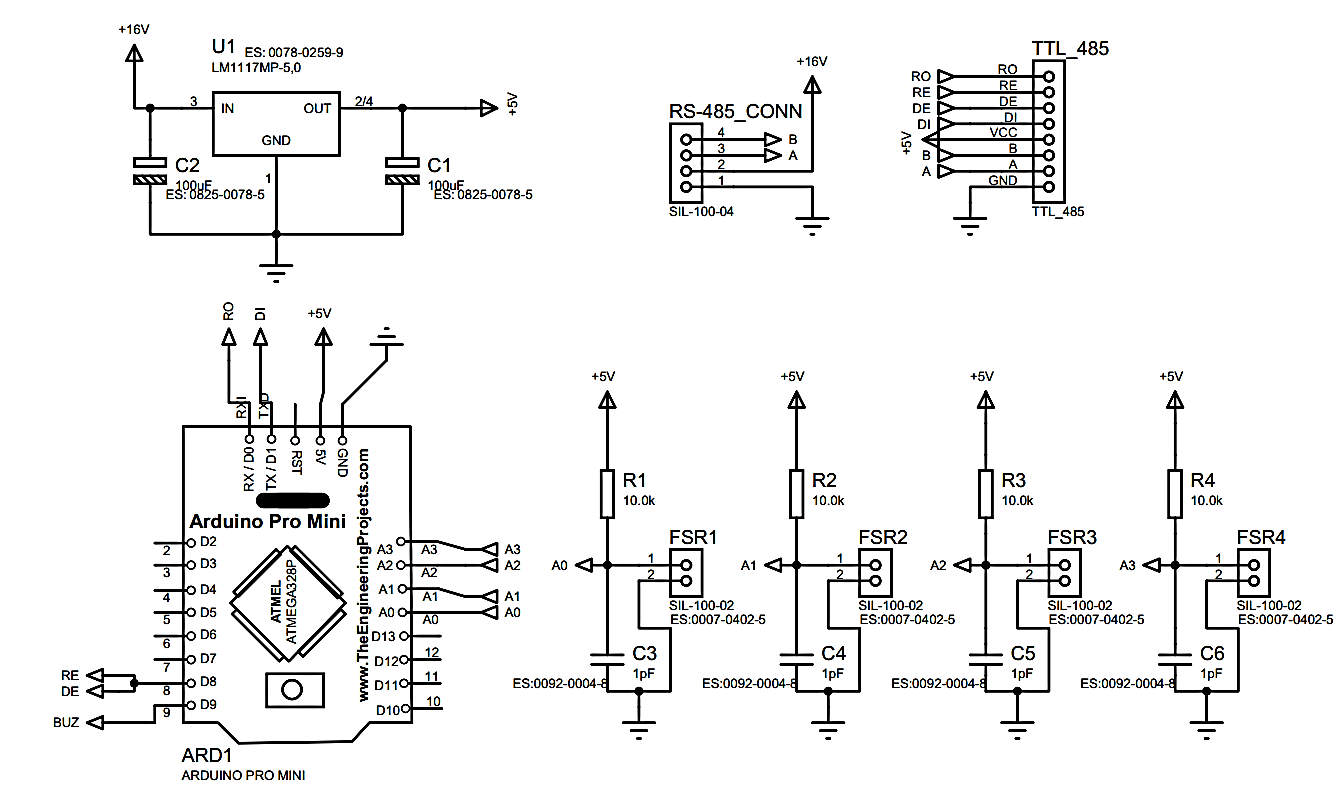
\includegraphics[width=0.8\textwidth]{chapter3/images/FSR_schematic.png}
  \caption{Schematic ของวงจร Ground Contact Sensor}
  \label{fig:FSR_schematic}
\end{figure}

\begin{figure}[!ht]
  \centering
  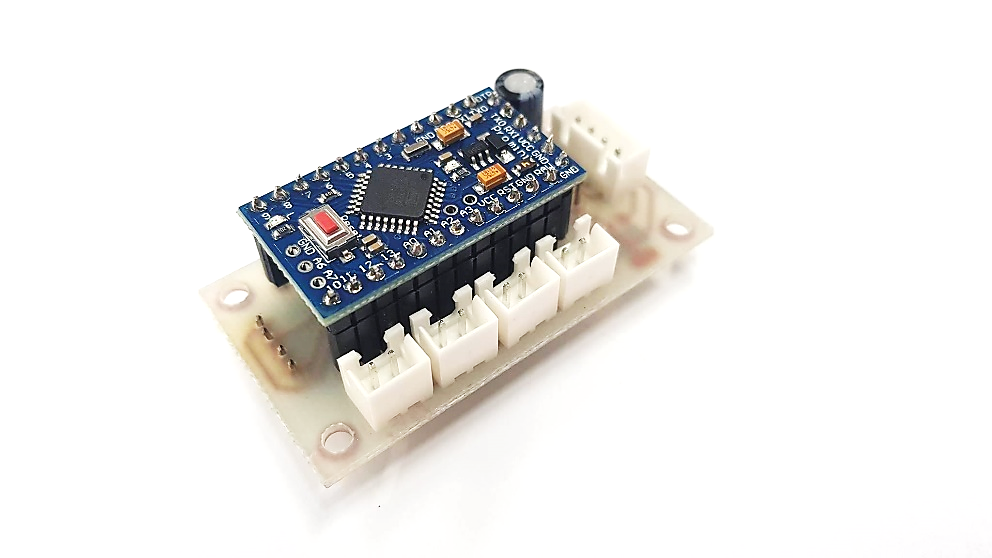
\includegraphics[width=0.8\textwidth]{chapter3/images/complete_FSR.png}
  \caption{แผงวงจร Ground Contact Sensor ที่ประกอบเสร็จแล้ว}
  \label{fig:complete_FSR}
\end{figure}

% \clearpage
% เซนเซอร์ที่เลือกใช้คือ Force Sensitive Resistor (FSR) เป็นเซนเซอร์ที่มีค่าความต้านทานภายในตัวเอง โดยเซนเซอร์นี้มีหลักการทำงานคือ 
% ค่าความต้านทานทางไฟฟ้าของตัวเซนเซอร์จะเปลี่ยนแปลงเมื่อมีแรงเข้ามากระทำกับหน้าสัมผัส เมื่อมีแรงเข้ามากระทำมาก จะทำให้ค่าความต้านทานต่ำ 
% หากไม่มีแรงเข้ามากระทำจะทำให้มีค่าความต้านทานสูง และเมื่อมีการนำเซนเซอร์นี้มาต่อกับตัวต้านทานที่มีค่าคงที่ ในรูปแบบของ Voltage Divider 
% ดังรูปที่ \ref{fig:FSR_schematic} จะทำให้สามารถอ่านค่าแรงดันไฟฟ้าที่เปลี่ยนแปลงตามแรงที่เกิดขึ้นกับหน้าสัมผัสของเซนเซอร์ FSR ได้ 

% \begin{figure}[!ht]
%   \centering
%   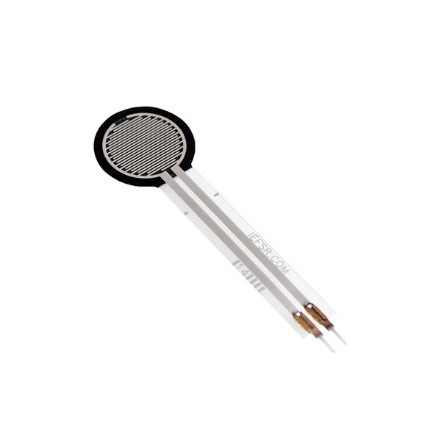
\includegraphics[width=0.3\textwidth]{chapter3/images/FSR.jpg}
%   \caption{Force Sensitive Resistor (FSR) ขนาด 0.5 นิ้ว}
%   \label{fig:FSR}
% \end{figure}

% ข้อดีของ FSR นั้นคือ เป็นเซนเซอร์ที่ถูกพัฒนาและออกแบบมาเพื่อใช้สำหรับการวัดแรงโดยตรง จึงทำให้ใช้งานได้ง่าย และสะดวก ในราคาที่ถูกกว่า 
% เมื่อเทียบกับเซนเซอร์ Load cell ที่มีราคาสูงและการใช้งานจำเป็นที่จะต้องมีวงจรขยายสัญญาณที่ใช้ในการอ่านค่าการบิดของวัสดุจาก 
% แต่ FSR นั้นก็มีข้อเสียเช่นกันคือ ความไม่ทนทานต่อการขีดข่วน เนื่องจากตัวเซนเซอร์ถูกทำมาจากฟิล์มพลาสติกบางๆ ซึ่งหากเกิดการขีดข่วนเกิดขึ้นแล้วอาจทำให้ฟิล์มฉีกขาดได้ 
% หากฟิล์มขาดจะทำให้ค่าความต้านทานออกมาไม่เหมือนเดิม ดังนั้นทางผู้เขียนจึงเลือกที่จะออกแบบโครงครอบสำหรับเซนเซอร์ FSR เพื่อป้องกันจากการถูกขีดข่วนจากภายนอก







%%%%%%%%%%%%%%%%%%%%%%%%%%%%%%%%%%%%%%%%%%%%%%%%%%%%%%%%%%%%%%%%%%%%%%%%%%%%%%%
\clearpage
\subsection{การเชื่อมต่อดิจิตอลเซอร์โวและเซนเซอร์}
โครงสร้างของหุ่นยนต์ฮิวมานอยด์ UTHAI มีขาสองข้างทำให้เกิดองศาอิสระ 12 องศาอิสระ
ผู้วิจัยจึงใช้ดิจิตอลเซอร์โวทั้งหมด 12 ตัว ดิจิตอลเซอร์โวทุกตัวเชื่อมต่อกันแบบสายโซ่เดซี่ (daisy chain) ดังรูปที่ \ref{fig:dynamixel_connect}
ข้างหนึ่งของมอเตอร์ตัวแรกเชื่อมต่อกับแบตเตอร์รี่ 12V และอีกข้างต่อกับ USB2RS485 เพื่อต่อไปยังตัวประมวลผลระดับสูง (Odroid)
และเซนเซอร์หน่วยวัดความเฉื่อย กับเซนเซอร์ตรวจจับหน้าสัมผัสที่พื้นเชื่อมต่อกับตัวประมวลผลระดับต่ำ (Nucleo F411RE)
ดังรูปที่ \ref{fig:odroid2dynamixel}
\begin{figure}[!ht]
    \centering
    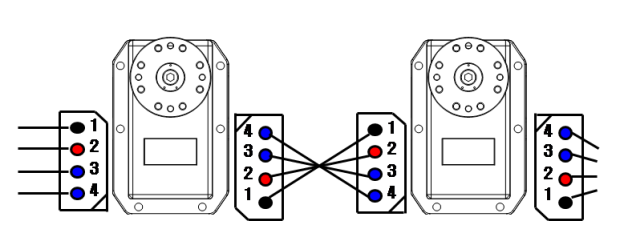
\includegraphics[width=0.8\textwidth]{chapter3/images/dynamixel_connect.png}
    \caption{การเชื่อมต่อกันระหว่างดิจิตอลเซอร์โว}
    \label{fig:dynamixel_connect}
\end{figure}
\begin{figure}[!ht]
    \centering
    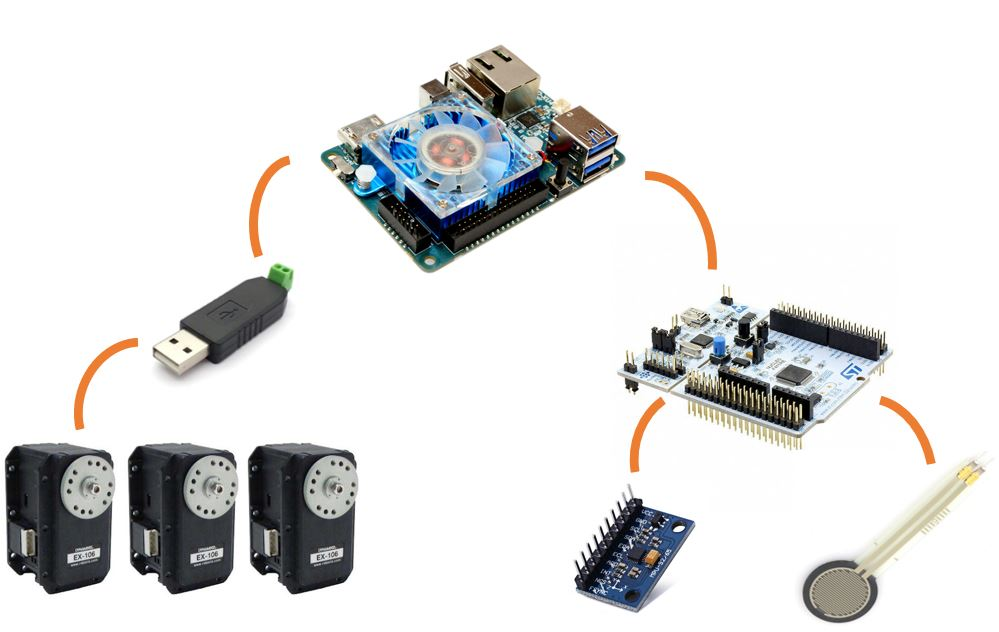
\includegraphics[width=0.9\textwidth]{chapter3/images/odroid2dynamixel.JPG}
    \caption{การเชื่อมต่อระหว่างตัวรับรู้ ตัวประมวลผล และตัวขับเคลื่อน}
    \label{fig:odroid2dynamixel}
\end{figure}


%%%%%%%%%%%%%%%%%%%%%%%%%%%%%%%%%%%%%%%%%%%%%%%%%%%%%%%%%%%%%%%%%%%%%%%%%%%%%%%
\clearpage
\subsection{การตั้งค่าดิจิตอลเซอร์โว}

\begin{wrapfigure}{l}{0.2\textwidth}
    
\includegraphics[width=0.9\linewidth]{chapter3/images/roboplus/roboplus.jpg} 
    \caption*{Roboplus 1.0}
\end{wrapfigure}

ก่อนที่จะเชื่อมต่อดิจิตอลเซอร์โวเข้ากับระบบประมวลผล จำเป็นที่จะต้องมีการตั้งค่า ID, Baudrate, Joint limited 
ของดิจิตอลเซอร์โว โดยการตั้งค่าพารามิเตอร์ของดิจิตอลเซอร์โวนั้น ผู้วิจัยจะใช้โปรแกรมที่มีชื่อว่า
Roboplus 1.0 ซึ่งเป็นเครื่องมือจากบริษัท Robotis ที่จำหน่ายดิจิตอลเซอร์โวนี้ โดยจะช่วยให้สามารถติดต่อกับดิจิตอลเซอร์โว
ตั้งค่าพารามิเตอร์ได้ แต่โปรแกรม Roboplus 1.0 นี้ใช้ได้เฉพาะใน Windows OS เท่านั้น ซึ่งสามารถดาวน์โหลดโปรแกรมได้จากหน้าเว็บไซต์ Robotis\footnote{http://www.robotis.us/roboplus1/}
เมื่อดาวน์โหลดโปรแกรมและติดตั้งเรียบร้อยแล้ว ให้เชื่อมต่อดิจิตอลเซอร์โวกับคอมพิวเตอร์ด้วย USB2RS485
และตั้งค่าพารามิเตอร์โดยทำตามขั้นตอน ดังรูปต่อไปนี้
\begin{figure}[!ht]
    \centering
    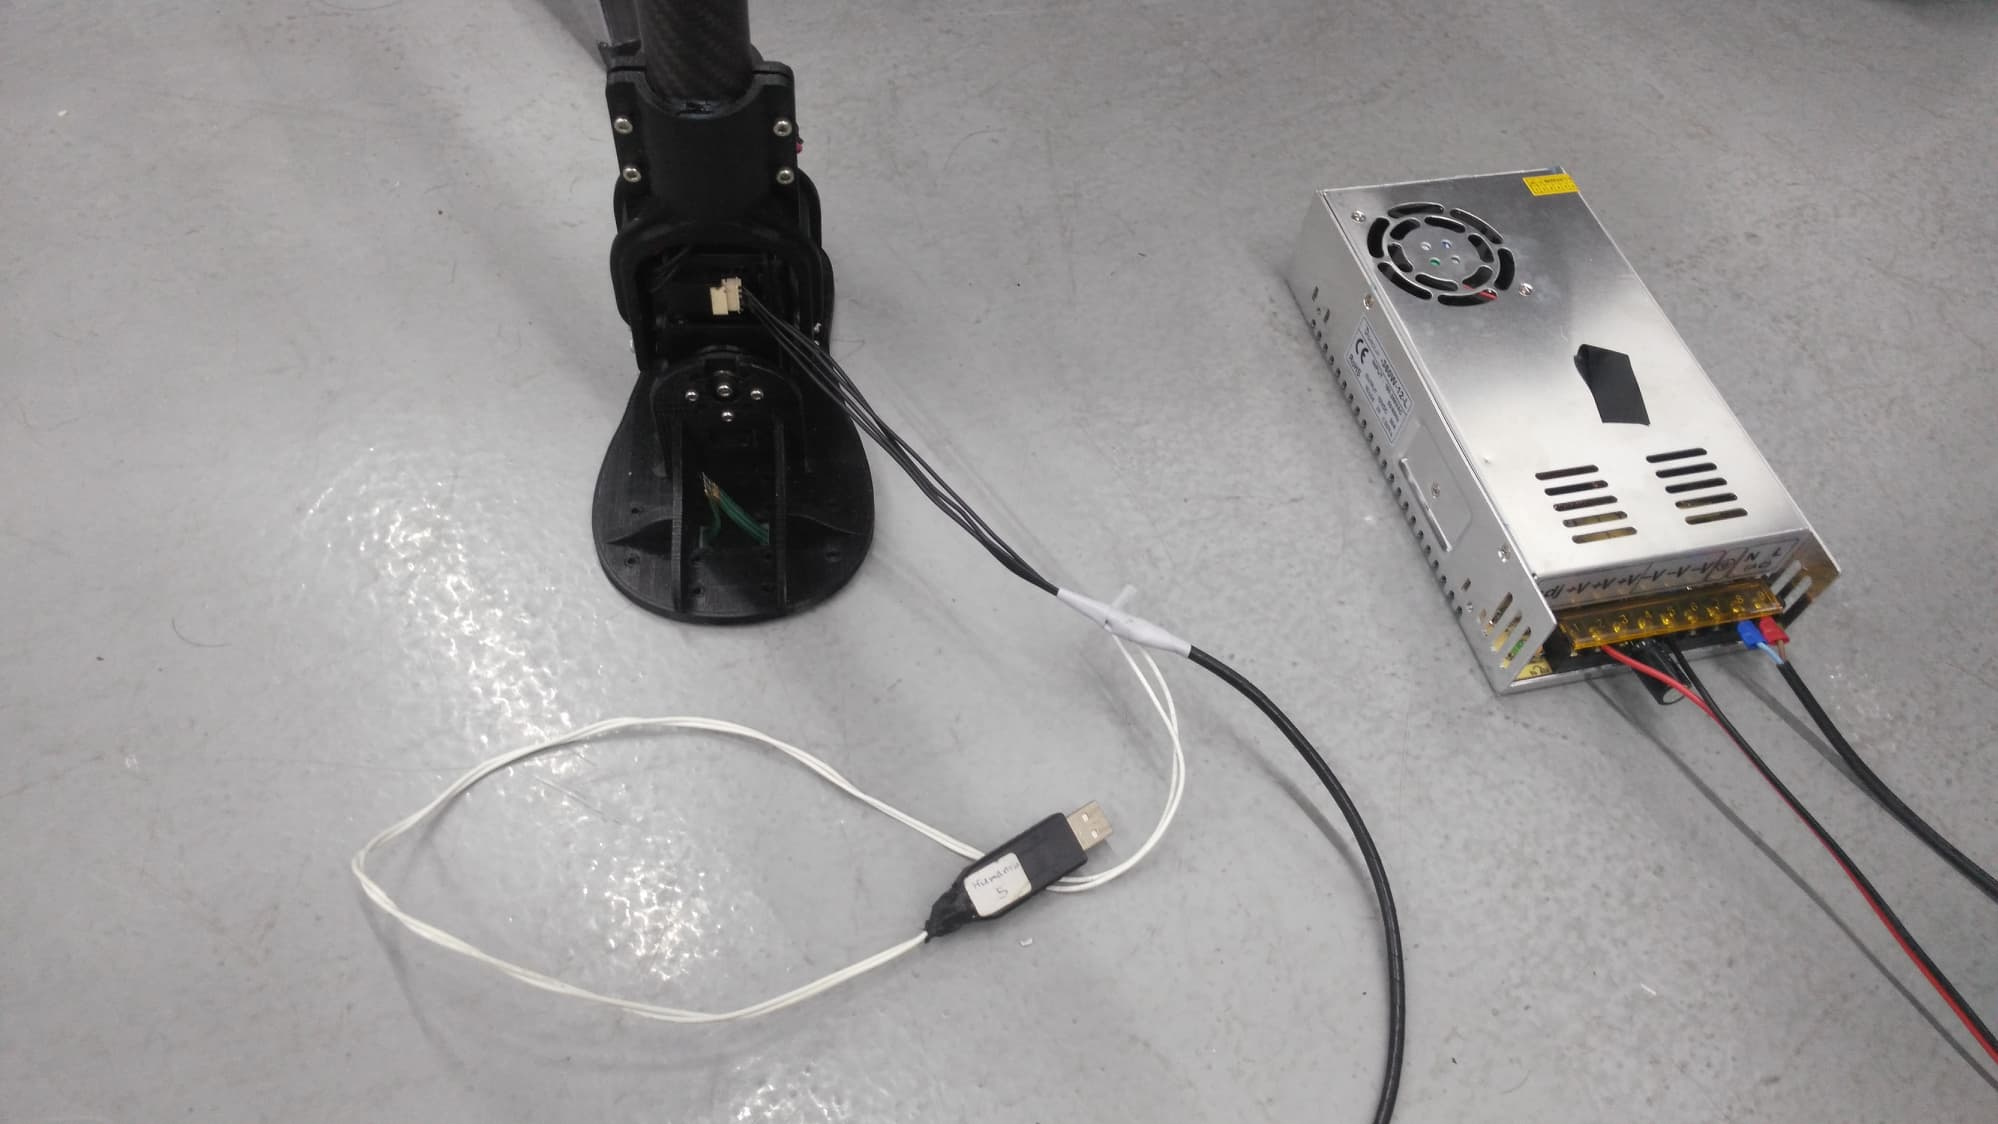
\includegraphics[width=\textwidth]{chapter3/images/roboplus/roboplus0.jpg}
    \caption*{เชื่อมต่อดิจิตอลเซอร์โวเข้ากับคอมพิวเตอร์ด้วย USB2RS485}
\end{figure}
\begin{figure}[!ht]
    \centering
    
\includegraphics[width=0.25\textwidth]{chapter3/images/roboplus/roboplus1.PNG}
    \caption*{เปิดโปรแกรม Roboplus 1.0}
\end{figure}
\begin{figure}[!ht]
    \centering
    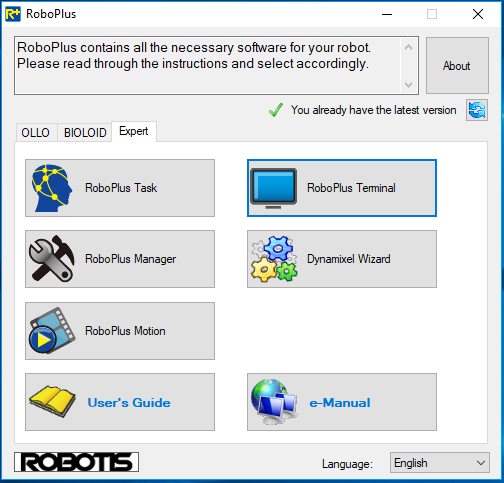
\includegraphics[width=0.55\textwidth]{chapter3/images/roboplus/roboplus2.PNG}
    \caption*{กดเข้าไปที่ Dynamixel Wizard}
\end{figure}
\begin{figure}[!ht]
    \centering
    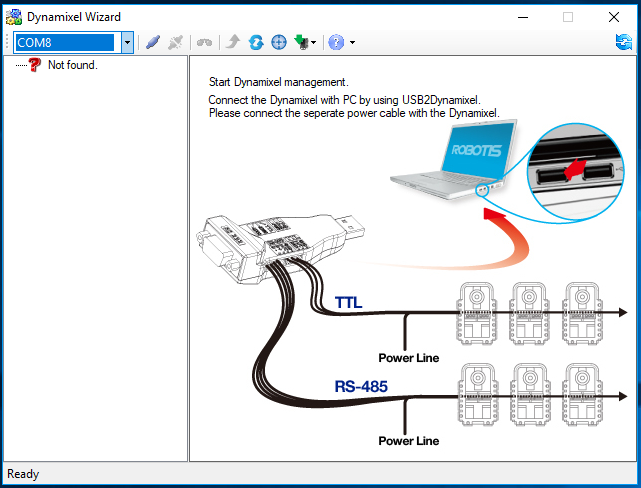
\includegraphics[width=0.55\textwidth]{chapter3/images/roboplus/roboplus3.PNG}
    \caption*{เลือก COM Port ให้ตรงกับ USB2RS485 จากนั้นกด Connect}
\end{figure}
\begin{figure}[!ht]
    \centering
    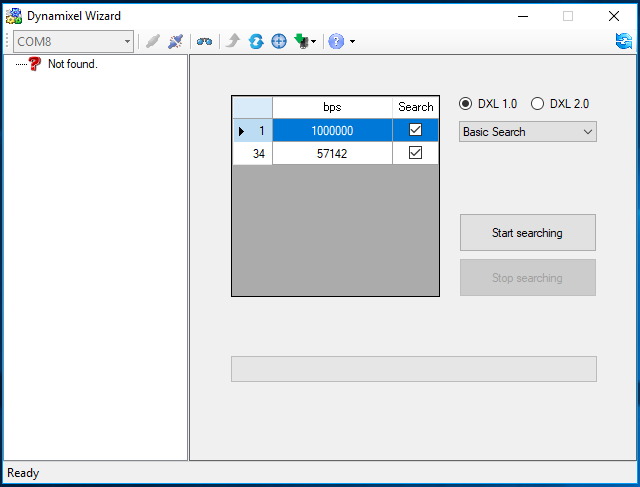
\includegraphics[width=0.55\textwidth]{chapter3/images/roboplus/roboplus4.PNG}
    \caption*{กดเลือกที่ช่อง 1Mbps แล้วกด Start searching}
\end{figure}
\begin{figure}[!ht]
    \centering
    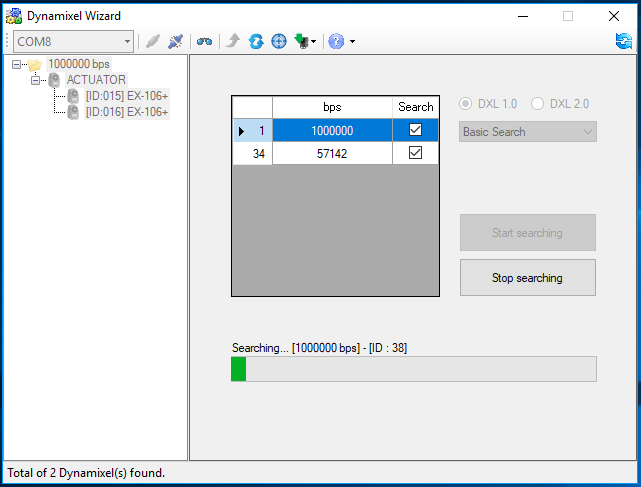
\includegraphics[width=0.55\textwidth]{chapter3/images/roboplus/roboplus5.PNG}
    \caption*{เมื่อเห็นทางด้านซ้ายมือโผล่ ID มอเตอร์ขึ้นมา หากขึ้นแล้วก็สามารถกด Stop Searching ได้}
\end{figure}
\begin{figure}[!ht]
    \centering
    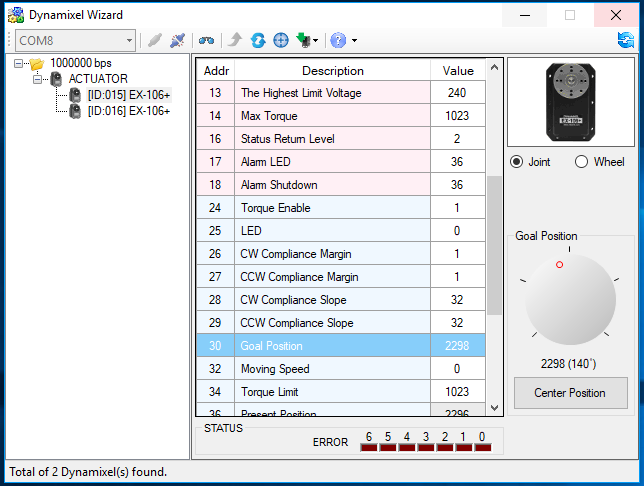
\includegraphics[width=0.55\textwidth]{chapter3/images/roboplus/roboplus6.PNG}
    \caption*{ทดสอบสั่งการมอเตอร์ที่ Addr 30 Goal position ว่าทิศทางถูกต้องหรือไม่}
\end{figure}
\begin{figure}[!ht]
    \centering
    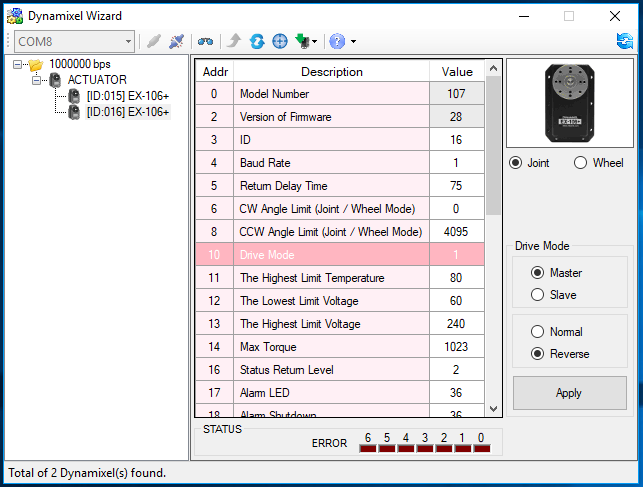
\includegraphics[width=0.55\textwidth]{chapter3/images/roboplus/roboplus7.PNG}
    \caption*{ถ้าทิศทางไม่ถูกต้องสามารถที่จะปรับได้ที่ Addr 10 Drive mode}
\end{figure}

%%%%%%%%%%%%%%%%%%%%%%%%%%%%%%%%%%%%%%%%%%%%%%%%%%%%%%%%%%%%%%%%%%%%%%%%%%%%%%%
\clearpage
\subsection{การเชื่อมต่อหน่วยประมวลผลระดับสูงและระดับต่ำ}
การเชื่อมต่อระหว่างหน่วยประมวลผล นั้นจะเชื่อมต่อกันผ่านสาย USB ชนิด Mini
และส่งข้อมูลหากันผ่าน Serial โดยใช้ rosserial นอกจากจะมีหน่วยประมวลผลแล้วยังมีบอร์ดที่เอาไว้ใช้สำหรับควบคุม
ดิจิตอลเซอร์โวเพื่อเผื่อเอาไว้สำหรับควบคุมการเคลื่อนไหวของแขนหุ่นยนต์ฮิวมานอยด์อุทัย
ดัวรูปที่ \ref{fig:uthai_controller} และทดสอบการสั่งการดังรูปที่ \ref{fig:uthai_drive} 

\begin{figure}[!ht]
    \centering
    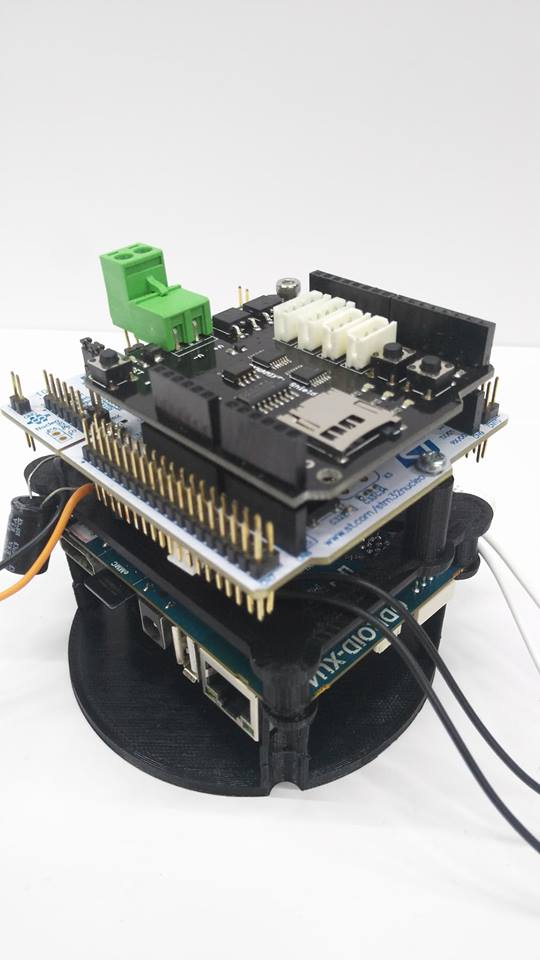
\includegraphics[width=0.4\textwidth]{chapter3/images/uthai_controller.jpg}
    \caption{การเชื่อมต่อกันระหว่างตัวประมวลผล}
    \label{fig:uthai_controller}
\end{figure}
\begin{figure}[!ht]
    \centering
    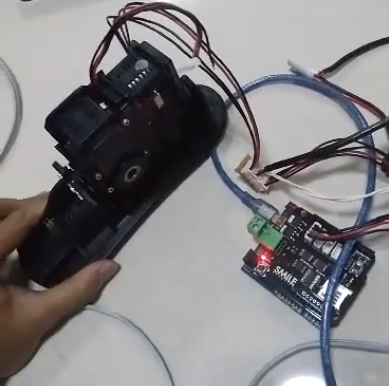
\includegraphics[width=0.5\textwidth]{chapter3/images/clean/uthai_drive.png}
    \caption{ตัวอย่างการใช้งานบอร์ดสั่งการดิจิตอลเซอร์โว}
    \label{fig:uthai_drive}
\end{figure}






\clearpage
\section{การออกแบบโปรแกรมด้วย ROS}
การออกแบบโปรแกรมด้วย ROS ของหุ่นยนต์ฮิวมานอยด์ UTHAI นั้น
ผู้วิจัยได้วางการทำงานโดย เริ่มจากการสร้างแบบจำลองเพื่อใช้ในการจำลองการทำงานของหุ่นยนต์ฮิวมานอยด์ UTHAI
โดยการจัดสร้างไฟล์ URDF ขึ้น ทดสอบการเคลื่อนไหวของหุ่นยนต์ในการแสดงผลด้วยภาพผ่านโปรแกรม RViz
ทดสอบการสั่งการดิจิตอลเซอร์โว ทดสอบการอ่านตำแหน่งจากดิจิตอลเซอร์โว
ทดสอบการส่งค่าตำแหน่งจากดิจิตอลเซอร์โวไปประมวลผลหาจุดศูนย์กลางมวลในโปรแกรม MATLAB
และเขียนโปรแกรมอ่านค่าเซนเซอร์ตรวจการสัมผัสพื้น

\vspace{20pt}
\subsection{กำหนดพิกัดเฟรมให้กับหุ่นยนต์ฮิวมานอยด์}
การกำหนดเฟรมให้กับหุ่นยนต์ฮิวมานอยด์ UTHAI นั้น ในวิทยานิพนธ์เล่มนี้ ผู้วิจัยจะใช้หลักตามของ
ROS Enhancement Proposals (REPs)\footnote{http://www.ros.org/reps/rep-0000.html}
ซึ่งการใช้หลักการนี้จะทำให้ การเขียนเป็นระบบระเบียบสามารถหยิบเครื่องมือต่างๆ
ที่สร้างขึ้นมาใช้งานร่วมกันได้ และช่วยทำให้เกิดความเข้าใจเวลาสื่อสาร

\paragraph*{base\_link}
เป็นเฟรมที่ติดอยู่กับฐานของหุ่นยนต์ฮิวมานอยด์ โดยจะติดตำแหน่งหรือมุมเอียงใดก็ได้
โดยส่วนใหญ่แล้วจะติดเฟรม base\_link ไว้ที่สะโพกของหุ่นยนต์

\paragraph*{base\_footprint}
เป็นเฟรมที่แสดงว่าหุ่นยนต์อยู่ตรงไหนเมื่อเทียบกับโลก โดยจะมีระดับอยู่ที่จุดต่ำสุดของฝ่าเท้า $z = min(l\_sole\_z,r\_sole\_z)$
โดย $l\_sole\_z$ และ $r\_sole\_z$ คือความสูงของฝ่าเท้า

\paragraph*{l\_wrist, r\_wrist}
เป็นเฟรมที่บอกตำแหน่งและมุมเอียงของแขนซ้ายและขวาของหุ่นยนต์ฮิวมานอยด์ โดยไม่ต้องคำนึงถึงการติดตั้งอุปกรณ์ใดๆเข้าไปที่ปลายแขนของหุ่นยนต์ฮิวมานอยด์

\paragraph*{l\_gripper, r\_gripper}
เป็นเฟรมที่บอกตำแหน่งและมุมเอียงของที่ปลายแขน (End effector) ถ้ามือจับอุปกรณ์อยู่ เฟรมนี้จะใช้ในการอ้างอิงตำแหน่งของอุปกรณ์นั้นๆ
แต่ในวิทยานิพนธ์นี้ ไม่ได้ใช้แขนของหุ่นยนต์ในการหยิบจับเครื่องมือหรือวัตถุ จึงไม่ได้ใช้เฟรมนี้

\paragraph*{l\_ankle, r\_ankle}
เป็นเฟรมที่บอกตำแหน่งและมุมเอียงของขาซ้ายและขวาโดยไม่ได้คำนึงว่าจุดรับน้ำหนักของตัวอยู่ที่ไหน

\paragraph*{l\_sole, r\_sole}
เป็นเฟรมที่บอกตำแหน่งและมุมเอียงของขาซ้ายและขวาที่รองรับน้ำหนักตัวอยู่
โดยจะบอกการฉายลงในระนาบของ $X$, $Y$ ที่สัมผัสพื้นและ $Z$ จะอยู่ระดับเดียวกับพื้นสัมผัส

\paragraph*{l\_toe, r\_toe}
เป็นเฟรมที่บอกตำแหน่งและมุมเอียงของปลายเท้าซ้ายและขวา

\paragraph*{gaze}
เป็นเฟรมที่บอกตำแหน่งและมุมเอียงของหัว โดยการเอียงนั้นจะบอกทิศทางของหัว โดยไม่ได้สนใจเซนเซอร์ว่าจะติดตั้งอย่างไร
แต่ในวิทยานิพนธ์นี้ หุ่นยนต์ฮิวมานอยด์ UTHAI ไม่มีหัว จึงไม่ได้ใช้เฟรมนี้

\paragraph*{torso}
เป็นเฟรมที่ติดอยู่กับลำตัวช่วงล่างของหุ่นยนต์ฮิวมานอยด์ โดยจะเป็นเฟรมที่ใช้เชื่อม ขา แขน ตัว หัว เข้าเอาไว้ด้วยกัน





%%%%%%%%%%%%%%%%%%%%%%%%%%%%%%%%%%%%%%%%%%%%%%%%%%%%%%%%%%%%%%%%%%%%%%%%%%%%%%%
\clearpage
\subsection{การแปลงข้อมูลให้อยู่ในรูปแบบ URDF}
เมื่อออกแบบโครงสร้างของหุ่นยนต์ฮิวมานอยด์ UTHAI ด้วยโปรแกรม Solidworks เสร็จแล้ว
ต่อไปเป็นการนำเอาไฟล์ STL ออกมาเพื่อใช้ในการทำระบบจำลองการทำงานของหุ่นยนต์
โดยการใช้งานระบบจำลองเนื่องจากทำให้ผู้วิจัยสามารถที่จะเห็นการทำงานของหุ่นยนต์ฮิวมานอยด์ได้
การสร้างแบบจำลองโดยการใช้เครื่องมือที่มาพร้อมกับ ROS ด้วยโมดูล URDF

\subsubsection{แพกเกจ ROS สำหรับสร้างแบบจำลอง}
ROS ได้ให้เครื่องมือที่ช่วยให้ สามารถที่จะสร้างแบบจำลองของหุ่นยนต์ฮิวมานอยด์สามมิติได้
เครื่องมือใน ROS ที่ชื่อว่า robot\_model ภายในมีแพกเกจต่างๆที่ใช้สำหรับสร้างแบบจำลองของหุ่นยนต์สามมิติอยู่อย่างครบถ้วน
ทำให้เราสามารถทำงานได้สะดวก และรวดเร็วมากขึ้น

\paragraph*{urdf}
เป็นหนึ่งในหลายแพกเกจที่อยู่ใน robot\_model, URDF เป็นไฟล์ XML ที่เอาไว้ใช้บอกลักษณะทางกายภาพของหุ่นยนต์ ซึ่งย่อมาจาก Unified Robot Description Format (URDF)
การบอกโครงสร้างของหุ่นยนต์ด้วย URDF จะใช้การบอกเป็นโครงสร้างต้นไม้ของก้านต่อต่างๆในตัวหุ่นยนต์

\paragraph*{joint\_state\_publisher}
เครื่องมือนี้มีประโยชน์มากในการสร้างแบบจำลองหุ่นยนต์ด้วย URDF เนื่องจากสามารถนำตำแหน่งของข้อต่อ มาแสดงเป็น GUI ได้ ทำให้เราสามารถเลื่อนๆหมุนๆไปมาได้ อีกทั้งยังสามารถใช้งานร่วมกับโปรแกรมแสดงผลภาพ RViz ได้

\paragraph*{robot\_state\_publisher}
เป็นเครื่องมือที่ใช้ในการ publish ตำแหน่งของก้านต่อต่างๆในแบบจำลองของหุ่นยนต์ฮิวมานอยด์ออกมาใน TF อีกทั้งยังให้ความสัมพันธ์ระหว่างเฟรมของหุ่นยนต์ได้ด้วย

\paragraph*{xacro}
ย่อมาจาก XML Macros หรือเราสามารถเรียกอีกอย่างว่าเครื่องมือเสริมสำหรับ URDF ซึ่งลักษณะการเขียนเหมือนกับไฟล์ URDF แต่การเขียนนั้นจะสั้นกว่า อ่านง่ายกว่า และสามารถใช้เพื่อทำให้สร้างหุ่นยนต์ที่มีความซับซ้อนง่ายขึ้น
สามารถแปลงไฟล์ xacro เป็น urdf ได้ถ้าต้องการ

\vspace{20pt}
\subsubsection{URDF}
ในส่วนนี้จะเป็นการอธิบายระบบทางกลของหุ่นยนต์ฮิวมานอยด์เป็นไฟล์ที่ใช้ร่วมกับ ROS
เพื่อที่จะสามารถนำไปใช้กับระบบจำลองการทำงานของหุ่นยนต์ในอนาคตได้
ในการอธิบายระบบทางกลนั้นผู้วิจัยได้ใช้ไฟล์ URDF ซึ่งใช้ภาษาการเขียนเป็น XML ในการบอกส่วนประกอบแต่ละส่วนของหุ่นยนต์

\subsubsection*{Link}
ในไฟล์ URDF แต่ละชิ้นส่วนของหุ่นยนต์เราจะเรียกว่า link แล้วใน link จะประกอบไปด้วยส่วนย่อยๆ
3 ส่วนคือ <inertia> ที่เอาไว้บอกถึงค่าตัวแปรทางฟิสิกส์, <visual> ที่เอาไว้แสดงผลให้เราเห็น, 
<collision> ที่เอาไว้ตรวจสอบว่าหุ่นยนต์มีการชนกันกับสิ่งแวดล้อมไหม ดังรูปที่ \ref{fig:urdf_link_code}

\clearpage
\begin{figure}[!ht]
\begin{Verbatim}[fontsize=\small]
<link name="my_link">
    <inertia>
        <origin xyz="0 0 0.5" rpy="0 0 0"/>
        <mass value="1"/>
        <inertia ixx="100" ixy="0" ixz="0" iyy="100" iyz="0" izz="100"/>
    </inertia>
    <visual>
        <origin xyz="0 0 0" rpy="0 0 0"/>
        <geometry>
            <box size="1 1 1" />
        </geometry>
        <material name="Cyan">
            <color rgba="0 1.0 1.0 1.0"/>
        </material>
    </visual>
    <collision>
        <origin xyz="0 0 0" rpy="0 0 0"/>
        <geometry>
            <cylinder radius="1" length="0.5"/>
        </geometry>
    </collision>
</link>
\end{Verbatim}
\caption{ตัวอย่าง link ใน urdf}
\label{fig:urdf_link_code}
\end{figure}

ยังมีอีกหลายตัวที่ใช้ในการอธิบายแต่ละชิ้นส่วนของหุ่นยนต์ แต่ตัวอย่างเป็นเพียงแค่ส่วนหนึ่งเท่านั้น
ในความเป็นจริงแล้วเราจะเขียน tags ต่างๆก็ตามที่เราต้องการ โดยใน URDF ไฟล์นั้นจะเอาไว้เก็บข้อมูลลักษณะเฉพาะของหุ่นยนต์เอาไว้
และยังสามารถใช้กับซอฟแวร์ตัวอื่นๆอีกได้\footnote{http://wiki.ros.org/urdf}
\begin{figure}[!ht]
	\centering
	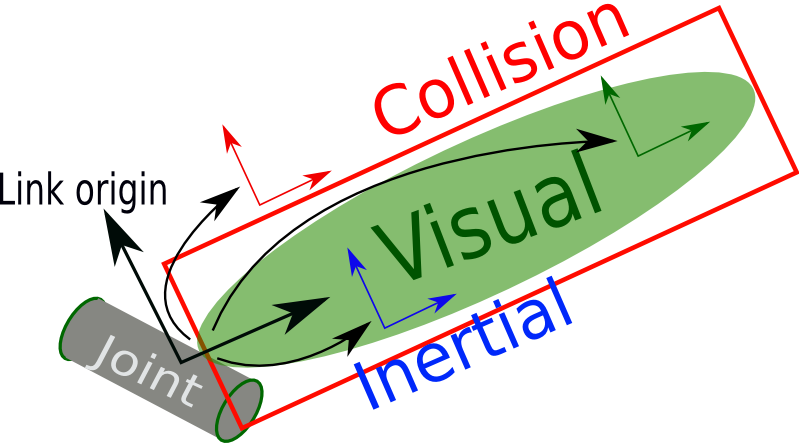
\includegraphics[width=0.60\textwidth]{chapter3/images/urdf_link.png}
	\caption{การอธิบาย link ใน URDF ไฟล์}
	\label{fig:urdf_link}
\end{figure}

\clearpage
\subsubsection*{Joint}
อีกส่วนที่สำคัญสำหรับการสร้างไฟล์หุ่นยนต์ด้วย URDF ก็คือ Joint tag โดย tag นี้จะอธิบายถึงความสัมพันธ์ระหว่างก้านต่อสองอัน
ส่วนนี้ไม่ได้มีเพียงแค่ทำข้อต่อให้เป็นแบบหมุนได้อย่างเดียว ยังมี Fix, Revolution, Linear และ Planar นอกเหนือจากนี้
เรายังสามารถที่จะเพิ่มองศาสูงสุดต่ำสุดของข้อต่อ รวมไปถึง dynamic properties ต่างๆ ตามที่เห็นดังรูปที่ \ref{fig:urdf_joint_code}
\begin{figure}[!ht]
\begin{Verbatim}[fontsize=\small]
<joint name="my_joint" type="floating">
	<origin xyz="0 0 1" rpy="0 0 3.1416"/>
	<parent link="link1"/>
	<child link="link2"/>
	<calibration rising="0.0"/>
	<dynamics damping="0.0" friction="0.0"/>
	<limit effort="30" velocity="1.0" lower="-2.2" upper="0.7"/>
	<safety_controller k_velocity="10" k_position="15" 
	soft_lower_limit="-2.0" soft_upper_limit="0.5"/>
</joint>
\end{Verbatim}
\caption{ตัวอย่าง joint ใน urdf}
	\label{fig:urdf_joint_code}
\end{figure}

เมื่อเรานำ Joint และ Link มารวมกันเราจะต้องพิจารณาว่ามีวางรูปแบบเป็นไปตามรูปที่ \ref{fig:urdf_joint}
โดยจะมีระยะระหว่างแกนของแต่ละข้อต่อกับก้านต่อ ชิ้นส่วนแรกของการสร้างไฟล์ URDF จะมีชื่อว่า base\_link
และเฟรม origin จะเป็นเฟรมอ้างอิง เมื่อเราต่อ Joint เข้ากับ Link จะเรียกก้านต่อที่เอามาติดว่า parent
โดยเฟรม origin ของข้อต่อจะอยู่จุดเดียวกับเฟรม origin ของก้านต่อ ในสถานะเดียวกันก้านต่อที่นำมาต่อจากข้อต่อ
เราจะเรียกว่า child และเฟรม origin ของก้านต่อ child จะอยู่ที่จุดเดียวกับเฟรม origin ของข้อต่อ

\begin{figure}[!ht]
	\centering
	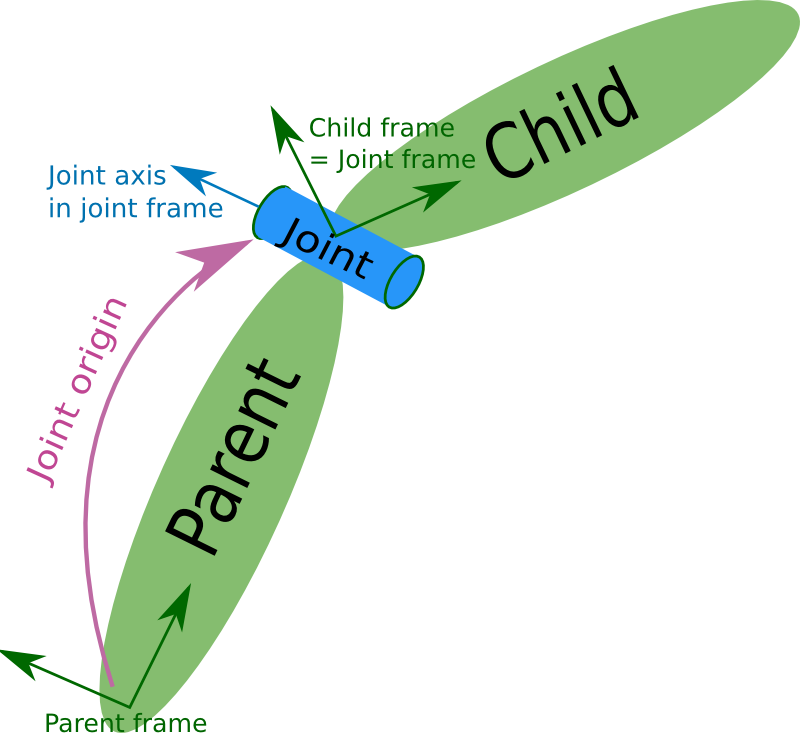
\includegraphics[width=0.55\textwidth]{chapter3/images/urdf_joint.png}
	\caption{การอธิบาย Joint ใน URDF ไฟล์}
	\label{fig:urdf_joint}
\end{figure}

%%%%%%%%%%%%%%%%%%%%%%%%%%%%%%%%%%%%%%%%%%%%%%%%%%%%%%%%%%%%%%%%%%%%%%%%%%%%%%%


%%%%%%%%%%%%%%%%%%%%%%%%%%%%%%%%%%%%%%%%%%%%%%%%%%%%%%%%%%%%%%%%%%%%%%%%%%%%%%%
%%%%%%%%%%%%%%%%%%%%%%%%%%%%%%%%%%%%%%%%%%%%%%%%%%%%%%%%%%%%%%%%%%%%%%%%%%%%%%%
\clearpage
\subsection{โครงสร้างการติดต่อสื่อสารระหว่าง Node ใน ROS}
การติดต่อสื่อสารกันภายใน ROS นั้นจะใช้การส่ง message หากัน ซึ่ง message แต่ละตัวก็จะใช้ในงานที่ต่างกัน
ตามระบบที่ต้องการส่ง จากรูปที่ \ref{fig:uthai_ros_node} เป็นโครงสร้างการส่งข้อมูลหากันของหุ่นยนต์ฮิวมานอยด์
ที่ผู้วิจัยได้ออกแบบไว้ โดยเริ่มจากผู้ใช้งานส่งตำแหน่งที่หุ่นยนต์จะต้องเดินไปไปยัง Node ที่ทำการคำนวณและสร้างตำแหน่งการวางเท้าของหุ่นยนต์
แล้วหลังจากนั้นจะส่งข้อมูลออกไปเป็น Path เส้นทางไปยัง Node ที่ทำการค้นหาตำแหน่งของ com, zmp ของหุ่นยนต์
เพื่อทำการควบคุมและสั่งการหุ่นยนต์ต่อไป

\begin{figure}[!ht]
	\centering
	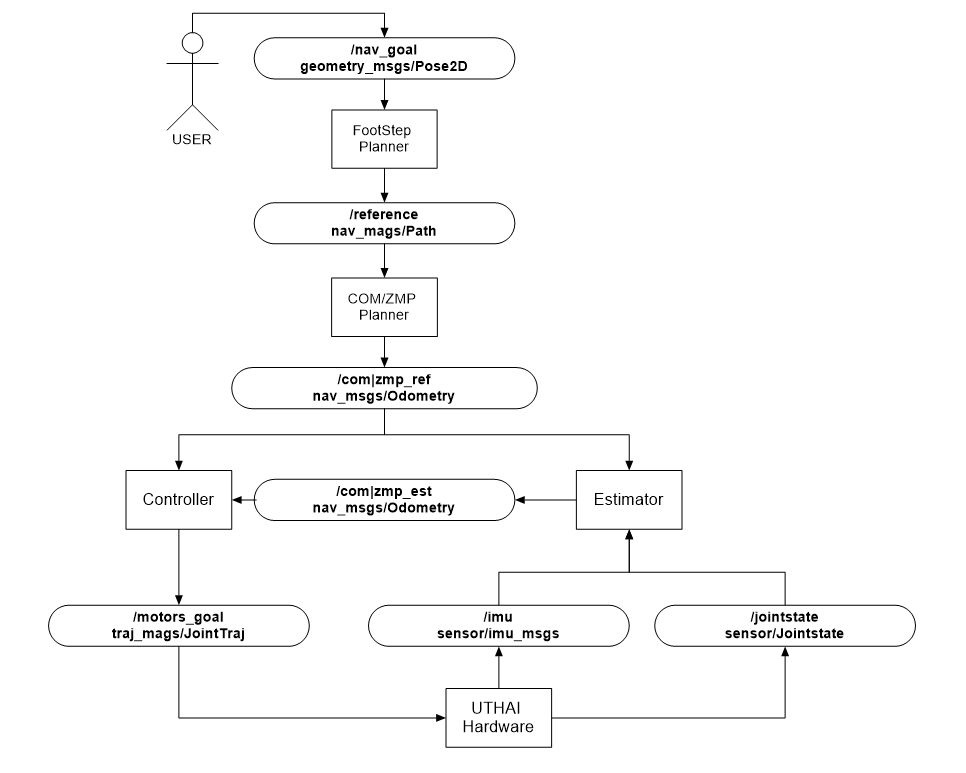
\includegraphics[width=\textwidth]{chapter3/images/uthai_ros_node.png}
	\caption{การติดต่อสื่อสารระหว่าง Node}
	\label{fig:uthai_ros_node}
\end{figure}

\subsubsection*{การบอกตำแหน่งและมุมเอียง}
การบอกตำแหน่งใน 3 มิติ Point คือการบอก $x$, $y$, $z$ และการบอกมุมเอียงจะใช้ Quaternion
ในการบอกโดยใช้ตัวแปรสี่ตัว คือ $x$,$y$,$z$,$w$ หากนำทั้งสองมารวมกันเราจะเรียกว่า Pose
\begin{table}[!ht]
	\centering
	\begin{tabular}{| c | c |}
		\hline
		\multicolumn{2}{|c|}{geometry\_msgs/Point}\\
		\hline
		float64 & x \\
		float64 & y \\
		float64 & z \\
		\hline
	\end{tabular}
	\caption{Message Geometry Point}
	\label{tab:geometry_point}
\end{table}
\begin{table}[!ht]
	\centering
	\begin{tabular}{| c | c |}
		\hline
		\multicolumn{2}{|c|}{geometry\_msgs/Quaternion}\\
		\hline
		float64 & x \\
		float64 & y \\
		float64 & z \\
		float64 & w \\
		\hline
	\end{tabular}
	\caption{Message Geometry Quaternion}
	\label{tab:geometry_quaternion}
\end{table}
\begin{table}[!ht]
	\centering
	\begin{tabular}{| c | c |}
		\hline
		\multicolumn{2}{|c|}{geometry\_msgs/Pose}\\
		\hline
		geometry\_msgs/Point & position \\
		geometry\_msgs/Quaternion & orientation \\
		\hline
	\end{tabular}
	\caption{Message Geometry Pose}
	\label{tab:geometry_pose}
\end{table}

\subsubsection*{การบอกความเร็วเชิงเส้นและเชิงมุม}
การบอกความเร็วเชิงเส้นใน 3 มิติ คือการบอกความเร็วตามแนวแกน $x$, $y$, $z$ และการบอกความเร็วเชิงมุม
คือการบอกความเร็วการหมุนรอบแกน $x$,$y$,$z$ หากนำทั้งสองมารวมกันเราจะเรียกว่า Twist
\begin{table}[!ht]
	\centering
	\begin{tabular}{| c | c |}
		\hline
		\multicolumn{2}{|c|}{geometry\_msgs/Vector3}\\
		\hline
		float64 & x \\
		float64 & y \\
		float64 & z \\
		\hline
	\end{tabular}
	\caption{Message Geometry Vector3}
	\label{tab:geometry_vector3}
\end{table}
\begin{table}[!ht]
	\centering
	\begin{tabular}{| c | c |}
		\hline
		\multicolumn{2}{|c|}{geometry\_msgs/Twist}\\
		\hline
		geometry\_msgs/Vector3 & linear \\
		geometry\_msgs/Vector3 & angular \\
		\hline
	\end{tabular}
	\caption{Message Geometry Twist}
	\label{tab:geometry_twist}
\end{table}

\subsubsection*{การบอกตำแหน่งและความเร็ว}
หากนำทั้งสองมารวมกันระกว่าง ตำแหน่ง (Pose) และความเร็ว (Twist) เราจะเรียกว่า Odometry
แต่ที่เพิ่มเข้ามาคือ Covariance ซึ่งอาจทำให้เกิดความสับสนได้
\begin{table}[!ht]
	\centering
	\begin{tabular}{| c | c |}
		\hline
		\multicolumn{2}{|c|}{nav\_msgs/Odometry}\\
		\hline
		std\_msgs/Header & header \\
		geometry\_msgs/PoseWithCovariance & pose \\
		geometry\_msgs/TwistWithCovariance & twist \\
		\hline
	\end{tabular}
	\caption{Message Navigation Odometry}
	\label{tab:nav_odometry}
\end{table}

\clearpage
\subsubsection*{ตำแหน่งของหุ่นยนต์}
การบอกตำแหน่งของหุ่นยนต์บนระนาบ 2 มิติ คือการบอก $x$, $y$ และ $\theta$
การบอกนั้นจะบอกว่าตำแหน่งที่หุ่นยนต์อยู่นั้นอยู่ตรงไหนหากเที่ยบกับแผนที่
รวมไปถึงตำแหน่งของหุ่นยนต์ที่ต้องการจะเดินไปด้วย ซึ่งอ้างอิงมาจากตำแหน่งเริ่มต้นของแผนที่ 
\begin{table}[!ht]
	\centering
	\begin{tabular}{| c | c |}
		\hline
		\multicolumn{2}{|c|}{geometry\_msgs/Pose2D}\\
		\hline
		float64 & x \\
		float64 & y \\
		float64 & theta \\
		\hline
	\end{tabular}
	\caption{Message Geometry Pose2D}
	\label{tab:geometry_pose2d}
\end{table}

\subsubsection*{ตำแหน่งการวางเท้าของหุ่นยนต์}
การจะให้หุ่นยนต์นำเท้าไปวางในตำแหน่งที่เราต้องการจากที่ได้จากการคำนวณนั้น
จะต้องบอกตำแหน่งและบอกมุมเอียงของจุดที่จะไป จากการสร้างจะได้เป็นรายการของเท้าซ้ายและขวา
โดยอิงจาก ตารางที่ \ref{tab:geometry_pose}
\begin{table}[!ht]
	\centering
	\begin{tabular}{| c | c |}
		\hline
		\multicolumn{2}{|c|}{nav\_msgs/Path}\\
		\hline
		std\_msgs/Header & header \\
		geometry\_msgs/PoseStamped[] & poses \\
		\hline
	\end{tabular}
	\caption{Message Navigation Path}
	\label{tab:nav_path}
\end{table}
\begin{table}[!ht]
	\centering
	\begin{tabular}{| c | c |}
		\hline
		\multicolumn{2}{|c|}{geometry\_msgs/PoseStamped}\\
		\hline
		std\_msgs/Header & header \\
		geometry\_msgs/Pose & pose \\
		\hline
	\end{tabular}
	\caption{Message Geometry PoseStamped}
	\label{tab:geometry_posestamped}
\end{table}

\subsubsection*{ตำแหน่งจุดศูนย์กลางมวลของหุ่นยนต์}
ใน Message นี้ใช้อยู่ 2 ที่คือ Message ที่ได้จากการวางแผนของ Node CoM Planner และ Node CoM Estimator
โดยทั้งสองจุดใช้ Message เหมือนกันส่งไปยัง Controller เพื่อควบคุมท่าทางต่างๆของหุ่นยนต์ต่อไป
Message ที่ใช้คือ Message จากตารางที่ \ref{tab:nav_odometry}
\begin{table}[!ht]
	\centering
	\begin{tabular}{| c | c |}
		\hline
		\multicolumn{2}{|c|}{nav\_msgs/Odometry}\\
		\hline
		std\_msgs/Header & header \\
		geometry\_msgs/PoseWithCovariance & pose \\
		geometry\_msgs/TwistWithCovariance & twist \\
		\hline
	\end{tabular}
	\caption*{Message Navigation Odometry}
\end{table}

\clearpage
\subsubsection*{การควบคุมข้อต่อของหุ่นยนต์}
ในการควบคุมข้อต่อแต่ละข้อของหุ่นยนต์ฮิวมานอยด์นั้นจะใช้ Message trjectory\_msgs/JointTrajectory
ซึ่งสามารถส่ง ตำแหน่ง ความเร็ว ความเร่ง และ แรงบิด ไปได้ ทำให้หากต้องการเปลี่ยนระบบใหม่สามารถทำได้โดยง่าย

\begin{table}[!ht]
	\centering
	\begin{tabular}{| c | c |}
		\hline
		\multicolumn{2}{|c|}{trajectory\_msgs/JointTrajectory}\\
		\hline
		std\_msgs/Header & header \\
		string[] & joint\_names \\
		trajectory\_msgs\_msgs/JointTrajectoryPoint[] & points \\
		\hline
	\end{tabular}
	\caption{Message Trajectory JointTrajectory}
	\label{tab:trajectory_jointrajectory}
\end{table}
\begin{table}[!ht]
	\centering
	\begin{tabular}{| c | c |}
		\hline
		\multicolumn{2}{|c|}{trajectory\_msgs/JointTrajectoryPoint}\\
		\hline
		float64[] & positions \\
		float64[] & velocities \\
  		float64[] & accelerations \\
  		float64[] & effort \\
  		duration & time\_from\_start \\
		\hline
	\end{tabular}
	\caption{Message Trajectory JointTrajectoryPoint}
	\label{tab:trajectory_jointrajectorypoint}
\end{table}

\subsubsection*{ค่าเซนเซอร์ข้อต่อของหุ่นยนต์}
ที่ข้อต่อของหุ่นยนต์ฮิวมานอยด์มีเซนเซอรที่เอาไว้ใช้ในการอ่านค่าตำแหน่ง ความเร็ว และแรง อยู่ด้วย
เราสามารถที่จะใช้ Message sensor\_msgs/JointState สำหรับอ่านค่าตำแหน่ง ความเร็ว แรง
ของตัวขับเคลื่อนแล้วส่งให้ Estimater Node ได้
\begin{table}[!ht]
	\centering
	\begin{tabular}{| c | c |}
		\hline
		\multicolumn{2}{|c|}{sensor\_msgs/JointState}\\
		\hline
		std\_msgs/Header & header \\
		float64[] & position \\
		float64[] & velocity \\
		float64[] & effort \\
		\hline
	\end{tabular}
	\caption{Message Sensor JointState}
	\label{tab:sensor_jointstate}
\end{table}

\subsubsection*{ค่าเซนเซอร์ฝ่าเท้าของหุ่นยนต์}
ที่ฝ่าเท้าของหุ่นยนต์ฮิวมานอยด์มีเซนเซอรที่เอาไว้ใช้ในการอ่าน แรงกดที่ฝ่าเท้า ใช้ในการเอามาบอกว่าเท้าสัมผัสพื้นหรือไม่
\begin{table}[!ht]
	\centering
	\begin{tabular}{| c | c |}
		\hline
		\multicolumn{2}{|c|}{geometry\_msgs/Wrench}\\
		\hline
		geometry\_msgs/Vector3 & force \\
		geometry\_msgs/Vector3 & torque \\
		\hline
	\end{tabular}
	\caption{Message Geometry Wrench}
	\label{tab:geometry_wrench}
\end{table}

\clearpage
\subsubsection*{ค่าเซนเซอร์ IMU ของหุ่นยนต์}
เซนเซอร์ IMU เป็นเซนเซอร์ที่เอาไว้ใช้ในการวัด ความเร็วเชิงมุม และ ความเร่งเชิงเส้น
หากนำทั้งคู่มารวมกันจะสามารถที่จะแปลงให้วัดมุมเอียงของเซนเซอร์ได้ โดยจะใช้ Message
std\_msgs/Imu ในการส่งให้ Node Estimator จากตัวหุ่นยนต์
\begin{table}[!ht]
	\centering
	\begin{tabular}{| c | c |}
		\hline
		\multicolumn{2}{|c|}{sensor\_msgs/Imu}\\
		\hline
		std\_msgs/Header & header \\
		geometry\_msgs/Quaternion & orientation \\
		float64[9] & orientation\_covariance \\
		geometry\_msgs/Vector3 & angular\_velocity \\
		float64[9] & angular\_velocity\_covariance \\
		geometry\_msgs/Vector3 & linear\_acceleration \\
		float64[9] & linear\_acceleration\_covariance \\
		\hline
	\end{tabular}
	\caption{Message Sensor Imu}
	\label{tab:sensor_imu}
\end{table}
\begin{table}[!ht]
	\centering
	\begin{tabular}{| c | c |}
		\hline
		\multicolumn{2}{|c|}{sensor\_msgs/MegneticField}\\
		\hline
		std\_msgs/Header & header \\
		geometry\_msgs/Vector3 & magnetic\_field \\
		float64[9] & magnetic\_field\_covariance \\
		\hline
	\end{tabular}
	\caption{Message Sensor MegneticField}
	\label{tab:sensor_megneticfield}
\end{table}
%%%%%%%%%%%%%%%%%%%%%%%%%%%%%%%%%%%%%%%%%%%%%%%%%%%%%%%%%%%%%%%%%%%%%%%%%%%%%%%
%%%%%%%%%%%%%%%%%%%%%%%%%%%%%%%%%%%%%%%%%%%%%%%%%%%%%%%%%%%%%%%%%%%%%%%%%%%%%%%

\clearpage
\section{การออกแบบระบบพื้นฐาน}
\subsection{วางโครงสร้างของระบบพื้นฐาน}
โครงสร้างระบบพื้นฐานของหุ่นยนต์ฮิวมานอยด์ UTHAI เป็นการวางระบบให้ผู้วิจัยสามารถที่จะช่วยกันพัฒนาได้
และเพื่อทำให้มีความเป็นระบบระเบียบ ง่ายต่อการแก้ไข ปรับปรุง
ซึ่งผู้วิจัยได้ออกแบบส่วนการทำงานต่างๆออกเป็นสามส่วน ตามหน้าที่การทำงาน คือ

\subsubsection*{Hardware Devices}
เป็นส่วนของอุปกรณ์ฮาร์ดแวร์ที่ใช้งานกับหุ่นยนต์ฮิวมานอยด์ ยกตัวอย่างเช่น ตัวขับเคลื่อน กล้อง ไมโครโฟน ลำโพง
หรืออื่นๆ ซึ่งในส่วนนี้สามารถเปลี่ยนฮาร์ดแวร์จริงๆเป็นระบบจำลองได้

\subsubsection*{Hardware Services}
เป็นส่วนของซอฟต์แวร์ที่ช่วยทำให้อุปกรณ์ฮาร์ดแวร์สามารถติดต่อสื่อสารกับระบบพื้นฐานของหุ่นยนต์ฮิวมานอยด์ UTHAIได้
ซึ่งจะช่วยทำให้การส่งข้อมูลเป็นมาตรฐานเดียวกัน

\subsubsection*{Communication}
เป็นส่วนของการติดต่อสื่อสารระหว่างซอฟต์แวร์กับฮาร์ดแวร์ผ่านระบบพื้นฐานของหุ่นยนต์ฮิวมานอยด์ ซึ่งจะคอยจัดการให้ข้อมูลทุกอย่างสามารถเชื่อมต่อกันได้
\begin{figure}[!ht]
	\centering
	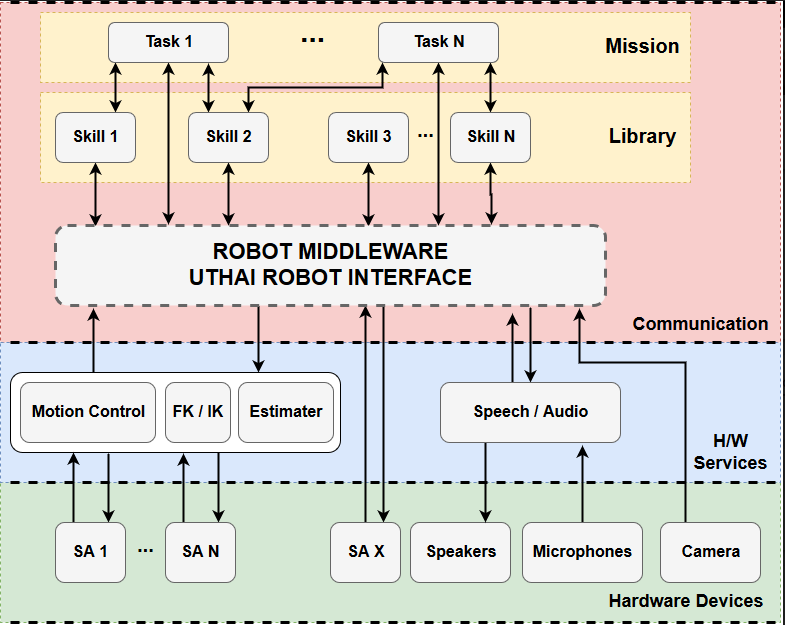
\includegraphics[width=0.8\textwidth]{chapter3/images/uthai_diagram.png}
	\caption{โครงสร้างพื้นฐานของหุ่นยนต์ฮิวมานอยด์ UTHAI}
	\label{fig:uthai_diagram}
\end{figure}

\clearpage
\begin{figure}[!ht]
	\centering
	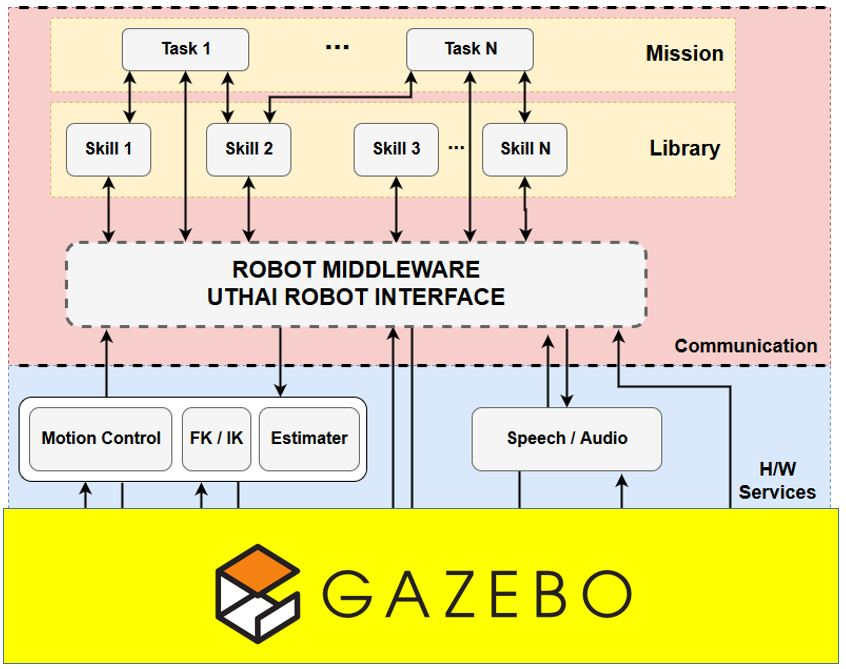
\includegraphics[width=0.85\textwidth]{chapter3/images/platform3.JPG}
	\caption{ภาพการเปลี่ยนส่วนของฮาร์ดแวร์เป็นระบบจำลอง}
\end{figure}
\begin{figure}[!ht]
	\centering
	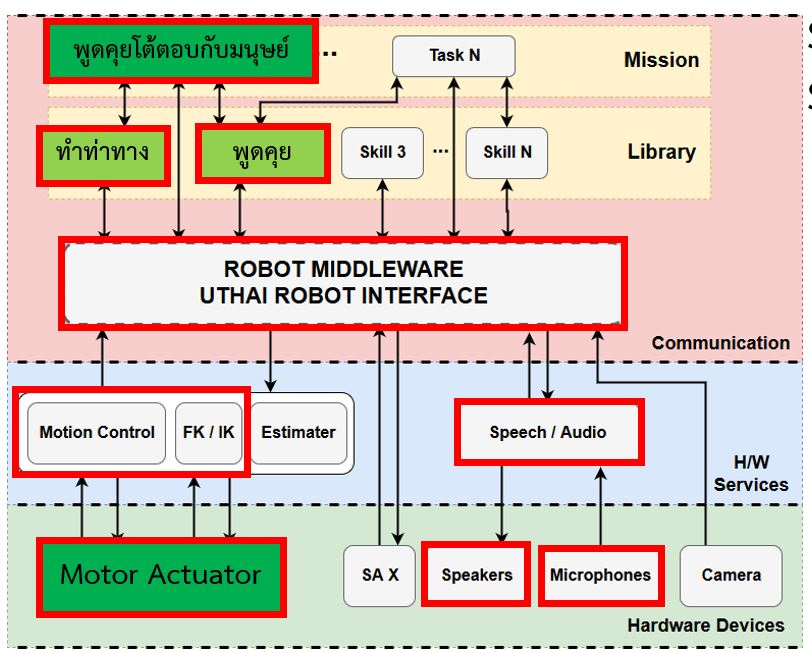
\includegraphics[width=0.85\textwidth]{chapter3/images/platform2.JPG}
	\caption{ตัวอย่างการนำโครงสร้างพื้นฐานไปประยุกต์ใช้ ในแอพลิเคชันการพูดคุยโต้ตอบกับมนุษย์}
\end{figure}

\clearpage
\subsection{ออกแบบสถาปัตยกรรมของหุ่นยนต์}
หลักการออกแบบสถาปัตยกรรมของหุ่นยนต์ฮิวมานอยด์ UTHAI จะออกแบบระบบให้อยู่บนระบบพื้นฐาน ROS
เนื่องจากการใช้กรอบการทำงานที่มีประสิทธิภาพ และความยืดหยุ่นสูง จะช่วยทำให้สามารถปรับเปลี่ยนระบบการควบคุมของหุ่นยนต์ฮิวมานอยด์ได้ง่ายและรวดเร็ว
การออกแบบหน่วยประมวลผลนั้นมีหลากหลายรูปแบบ ดังที่กล่าวไปในบทที่ 2 สำหรับในงานวิจัยครั้งนี้ผู้วิจัยได้ศึกษาและพบกว่าสถาปัตยกรรมที่เหมาะสมกับหุ่นยนต์ฮิวมานอยด์ UTHAI
จะมีลักษณะใกล้เคียงกับหุ่นยนต์ฮิวมานอยด์ Robotis OP3 ดังรูปที่ \ref{fig:op3_argitec} ดังนั้นแล้วผู้วิจัยจึงได้แบ่งการประมวลผลออกเป็น 2 ส่วนคือ
\begin{enumerate}[label=\arabic*, leftmargin=1.5cm]\setlength\itemsep{-0.25em}
	\item หน่วยประมวลผลควบคุมระดับสูง (High Level Controller)
	\item หน่วยประมวลผลควบคุมระดับต่ำ (Low Level Controller)
\end{enumerate}
\begin{figure}[!ht]
	\centering
	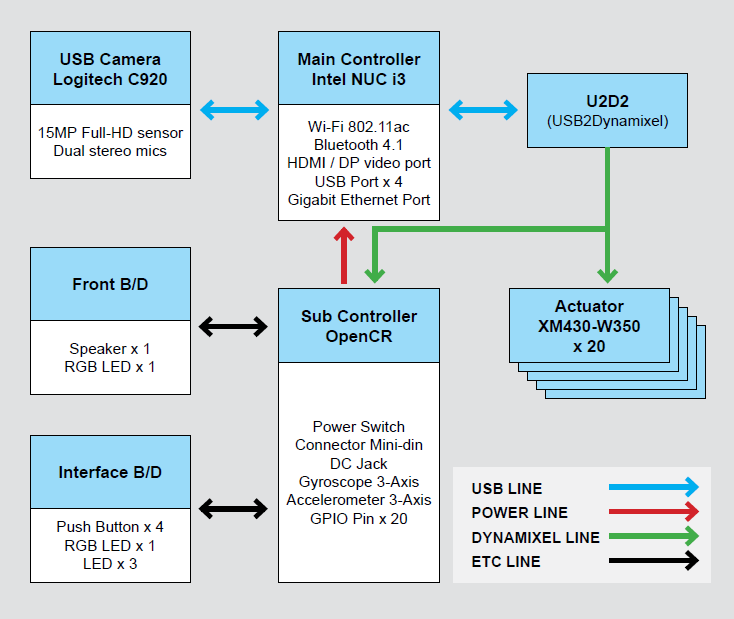
\includegraphics[width=0.6\textwidth]{chapter3/images/op3_029.png}
	\caption{สถาปัตยกรรมของหุ่นยนต์ Robotis OP3}
	\label{fig:op3_argitec}
\end{figure}
\begin{figure}[!ht]
	\centering
	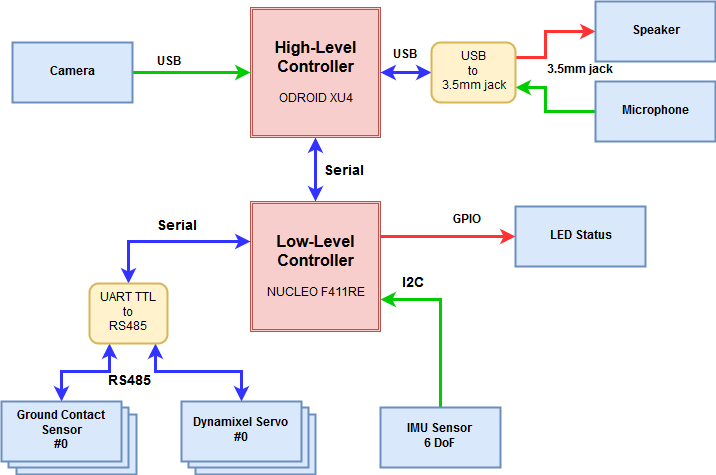
\includegraphics[width=0.7\textwidth]{chapter3/images/uthai_argitec.png}
	\caption{สถาปัตยกรรมของหุ่นยนต์ฮิวมานอยด์ UTHAI}
	\label{fig:uthai_argitec}
\end{figure}

\clearpage
\subsubsection{หน่วยประมวลผลควบคุมระดับสูง (High level controller)}
ระบบควบคุมหลักของหุ่นยนต์ฮิวมานอยด์ UTHAIนั้นจะอยู่ที่หน่วยประมวลผลขั้นสูง ใช้เป็นบอร์ดคอมพิวเตอร์ ODROID-XU4 ตัวประมวลผลหลักนี้
ทำหน้าที่ในการคำนวณเส้นทางการเดิน ทำให้หุ่นยนต์มีเสถียรภาพในการเดิน ตรวจการขัดกันของโครงสร้างของหุ่นยนต์
รวมไปถึงรับค่าข้อมูลตำแหน่ง ความเร็วจากข้อต่อ หลังจากนั้นจะทำการนำค่าทั้งหมดที่ได้จากการคำนวณ
มาแปลงให้อยู่ในรูปของชุดข้อมูล แล้วส่งออกไปให้ระบบกลาง (ROS) ในการส่งต่อไปให้อุปกรณ์อื่นต่อไป

\begin{figure}[ht]
	\centering
	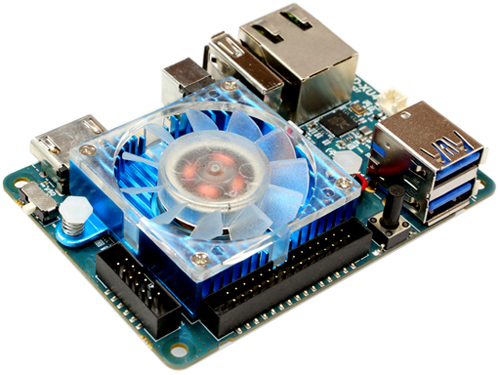
\includegraphics[width=0.45\textwidth]{chapter3/images/odroid_xu4.jpeg}
	\caption{บอร์ดคอนโทรลเลอร์ Odroid XU4}
	\label{fig:controller_xu4}
\end{figure}

\subsubsection{หน่วยประมวลผลควบคุมระดับต่ำ (Low level controller)}
ระบบควบคุมขั้นต่ำเป็นหน่วยประมวลผลที่รองลงมาจาก บอร์ดคอมพิวเตอร์ โดยใช้บอร์ดไมโครคอลโทรเลอร์ Nucleo F411RE
เป็นหน่วยประมวลผลขั้นต่ำ สำหรับในการติดต่อกับอุปกรณ์อิเล็กทรอนิกส์ต่างๆ ที่อยู่ภายในตัวของหุ่นยนต์ เช่น
ค่าเซนเซอร์ที่ฝ่าเท้าซึ่งสามารถบอกได้ว่าควรใช้สมการไหนในการคำนวณพลวัต หรือค่าของเซนเซอร์หน่วยวัดความเฉื่อยมีความสำคัญมาก
ในการทำให้หุ่นยนต์ฮิวมานอยด์เดินได้อย่างมีเสถียรภาพ เมื่ออ่านค่าเซนเซอร์ต่างๆได้แล้ว
หน่วยประมวลผลขั้นต่ำจะนำค่าที่ได้จากการอ่านเซนเซอร์เหล่านี้แปลงให้อยู่ในลักษณะของชุดข้อมูล แล้วส่งออกไปในระบบกลาง (ROS)
นอกเหนือจากนี้หน่วยประมวลผลขั้นต่ำยังทำหน้าที่รับค่าคำสั่งมาจากระบบกลาง ในการสั่งงานให้หุ่นยนต์มีท่าทางต่างๆได้

\begin{figure}[ht]
	\centering
	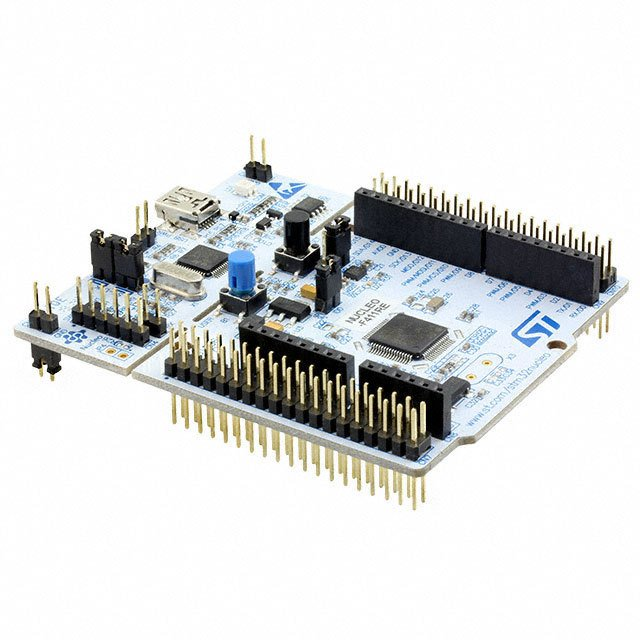
\includegraphics[width=0.45\textwidth]{chapter3/images/nucleo_f411re.jpeg}
	\caption{บอร์ดคอนโทรลเลอร์ Nucleo F411RE}
	\label{fig:controller_f411re}
\end{figure}


%%%%%%%%%%%%%%%%%%%%%%%%%%%%%%%%%%%%%%%%%%%%%%%%%%%%%%%%%%%%%%%%%%%%%%%%%%%%%%%

\clearpage
\subsection{จัดทำคู่มือและเอกสารการใช้งาน}
คู่มือจะเป็นส่วนที่ผู้มาพัฒนาต่อยอดสามารถที่จะอ่านทำความเข้าใจได้ โดยจะเขียนให้อยู่ในรูปของไฟล์ 
Markdown (.md) และเก็บเอาไว้ในเว็บไซท์ GitHub ซึ่งเป็นแหล่งรวม Source code ออนไลน์
สามารถเข้าไปดาวน์โหลดไฟล์ลงเครื่องผู้ใช้ แล้วทำการติดตั้งใช้งานได้เลย อีกทั้งผู้ใช้ยังสามารถส่ง Code
ของตัวเองเข้าระบบเพื่อช่วยพัฒนาและเพิ่มประสิทธิภาพในการทำงานของซอฟต์แวร์ของหุ่นยนต์ได้

% ส่วนที่ทำคู่มือและเอกสารเบื้องต้นคือ\vspace{-5mm}
% \begin{enumerate}[label=\arabic*, leftmargin=1.5cm]\setlength\itemsep{-0.25em}
% 	\item รายการวัสดุที่ใช้ในการทำหุ่นยนต์ฮิวมานอยด์ UTHAI
% 	\item รายละเอียดการเชื่อมต่อระหว่างอุปกรณ์ที่อยู่ในตัวหุ่นยนต์
% 	\item รายละเอียดการประกอบชิ้นส่วนทางกล
% 	\item รายละเอียดการใช้งานโปรแกรมพื้นฐาน
% \end{enumerate}

\subsubsection{รายการวัสดุที่ใช้ในการทำหุ่นยนต์ฮิวมานอยด์ UTHAI}
\begin{table}[ht]
	\centering
	\begin{tabular}{| l | c | c | c|}
		\hline
		รายการ & จำนวน (หน่วย) & บาท/หน่วย & ราคารวม(บาท) \\
		\hline
		===== Processing Unit & - & - & -\\
		Odroid XU4 Embeded Computer & 1 & 3800 & 3800\\
		Shifter Shield for Odoird XU4 & 1 & 1000 & 1000\\
		===== Sensor & - & - & -\\
		Force sensitive Resistor & 8 & 300 & 2400\\
		Electronic Component & 1 & 2000 & 2000\\
		MPU9255 9 Axis IMU Module & 1 & 500 & 500\\
		===== Structure & - & - & -\\
		อุปกรณ์ส่งกำลัง & 1 & 3000 & 3000\\
		ค่าวัสดุ เช่น Filament 3D printer , Carbon Fiber & 1 & 8000 & 8000\\
		สปริง & 14 & 50 & 700\\
		อุปกรณ์สิ้นเปลือง เช่น กระดาษทราย ฯลฯ & 1 & 1000 & 1000\\
		===== อุปกรณ์เสริม Motor Dynamixel & - & - & -\\
		Frame สำหรับต่อพ่วงมอเตอร์ & 4 & 2000 & 8000\\
		Horn Bearing & 4 & 1400 & 5600\\
		อุปกรณ์จ่ายพลังงาน & - & - & -\\
		Power Supply & 1 & 2000 & 2000\\
		Battery Li-Po 4 cell & 1 & 3000 & 3000\\
		===== รวม & - & - & 48000\\
		\hline
	\end{tabular}
	\caption{ตารางแสดงรายการของวัสดุต่าง ๆ}
	\label{tab:matrial_buyer}
\end{table}
ใช้สำหรับแจกแจงค่าใช้จ่ายเบื้องต้นเท่านั้น ไม่สามารถใช้อ้างอิงงบประมาณแบบละเอียดได้

%%%%%%%%%%%%%%%%%%%%%%%%%%%%%%%%%%%%%%%%%%%%%%%%%%%%%%%%%%%%%%%%%%%%%%%%%%%%%%%
% \subsubsection{รายละเอียดการเชื่อมต่อระหว่างอุปกรณ์ที่อยู่ในตัวหุ่นยนต์}
% \subsubsection{รายละเอียดการประกอบชิ้นส่วนทางกล}
% \subsubsection{รายละเอียดการใช้งานโปรแกรมพื้นฐาน}

